%%  'printversion' pro sazbu verze pro tisk (nebarevné logo a odkazy,
%%  odkazy s uvedením adresy za odkazem, ne odkazy do rejstříku),
%%  jinak verze pro prohlížeč

%%  'biblatex' pro zapnutí podpory pro sazbu bibliografie pomocí
%%  BibLaTeXu, jinak je výchozí sazba v prostředí thebibliography

%%  'language=jazyk' pro jazyk práce, jazyky english pro anglický,
%%  slovak pro slovenský, jinak je výchozí czech pro český

%%  'font=sans' pro bezpatkový font (Iwona Light), jinak je výchozí
%%  serif pro patkový (Latin Modern)

%%  'figures, tables, theorems a sourcecodes' pro sazbu seznamu
%%  obrázků, tabulek, vět a zdrojových kódů, jinak při =false se
%%  nesází (u theorems a sourcecodes výchozí)

\documentclass[
%  printversion,
  biblatex = false,
  language=english,
%  font=sans,
  figures=false,
%  tables=false,
  sourcecodes,
  glossaries,
  index
]{kidiplom}

%% Informace pro úvodní strany. V jazyku práce (pokud není v komentáři
%% uvedeno česky) a anglicky. Uveďte všechny, u kterých není v
%% komentáři uvedeno, že jsou volitelné. Při neuvedení se použijí
%% výchozí texty. Text pro jiný než nastavený jazyk práce (nepovinným
%% parametrem language makra \documentclass, výchozí český) se zadává
%% použitím makra s uvedením jazyka jako nepovinného parametru.

%% Název práce, česky a anglicky. Měl by se vysázet na jeden řádek.
\title[czech]{Vytvoření komplexní aplikace pro iOS pomocí SwiftUI a Swift Backend Development}
\title[english]{Building a comprehensive iOS application with SwiftUI and Swift Backend Development}

%% Jméno autora práce. Makro nemá nepovinný parametr pro uvedení
%% jazyka.
\author{Maksym Kupchenko}

%% Jméno vedoucího práce (včetně titulů). Makro nemá nepovinný
%% parametr pro uvedení jazyka.
\supervisor{Mgr. Roman Vyjídáček}

%% Volitelný rok odevzdání práce. Výchozí je aktuální (kalendářní)
%% rok. Makro nemá nepovinný parametr pro uvedení jazyka.
\yearofsubmit{2024}

%% Anotace práce, včetně anglické (obvykle překlad z jazyka
%% práce). Jeden odstavec!
\annotation[czech]{Závěrečná práce se zabývá vývojem serveru Vapor s PostgreSQL a mobilní aplikací SwiftUI pro iOS. Zahrnuje vývoj Swift na straně serveru, ověřování, ověřování dat a zpracování chyb. Práce hodnotí výkon, použitelnost a bezpečnost. Přispívá ke znalostem o Swift na straně serveru a ukazuje potenciál Vapor a SwiftUI pro škálovatelná řešení aplikací pro iOS.}

\annotation[english]{Bachelor thesis explores the development of a Vapor server with PostgreSQL and a SwiftUI iOS application. It covers server-side Swift development, authentication, data validation, and error handling. The work evaluates performance, usability, and security. It contributes to knowledge on server-side Swift, showcasing the potential of Vapor and SwiftUI for scalable iOS app solutions.}

%% Klíčová slova práce, včetně anglických. Oddělená (obvykle) středníkem.
\keywords[czech]{Mobilní aplikace;Swift; Vapor; SwiftUI; iOS; PostgreSQL}
\keywords[english]{Mobile application; Swift; Vapor; SwiftUI; iOS; PostgreSQL}

%% Volitelná specifikace příloh textu práce, i anglicky. Výchozí je
%% 'elektronická data v systému katedry informatiky / electronic data
%% in system of department of computer science'.
%\supplements{nejlepší software všech dob}
%\supplements[english]{the best software of all times}

%% Volitelné poděkování. Stručné! Výchozí je prázdné. Makro nemá
%% nepovinný parametr pro uvedení jazyka.

%% Cesta k souboru s bibliografií pro její sazbu pomocí BibLaTeXu
%% (zvolenou nepovinným parametrem biblatex makra
%% \documentclass). Použijte pouze při této sazbě, ne při (výchozí)
%% sazbě v prostředí thebibliography.
%\bibliography{bibliografie.bib}

%% Další dodatečné styly (balíky) potřebné pro sazbu vlastního textu
%% práce.
\usepackage{lipsum}
\usepackage{longtable}
\usepackage{graphicx}
\graphicspath{ {text/} }
\usepackage{placeins}

\begin{document}
%% Sazba úvodních stran -- titulní, s bibliografickými údaji, s
%% anotací a klíčovými slovy, s poděkováním a prohlášením, s obsahem a
%% se seznamy obrázků, tabulek, vět a zdrojových kódů (pokud jejich
%% sazba není vypnutá).
\maketitle

%% Vlastní text závěrečné práce. Pro povinné závěry, před přílohami,
%% použijte prostředí kiconclusions. Povinná je i příloha s obsahem
%% elektronických dat.

%% -------------------------------------------------------------------


\section{Introduction}

Today's trend is leaning towards mobile-first solutions, as mobile platforms offer faster and more intuitive user experiences. At present, there exist loads of web-based and multi-platform applications for task management, catering to the needs of users. However, there is a noticeable absence of a native mobile application.

My motivation arises from the need to streamline task management processes in school and provide users with a more convenient means of organizing their tasks effectively.

In this bachelor thesis, I aim to design and implement a server-side and iOS application focused on task management, named "StudentChrono". This application will empower users to easily create, update, track, and solve their tasks, and categorize them based on priority or deadline. "StudentChrono" will serve as a comprehensive tool for users to manage their tasks efficiently.

In the first chapter, I look into the theoretical basis and technologies needed to create the iOS platform's application development, architecture, and programming paradigm in addition to other patterns utilized in server-side and mobile development. I analyze services that are appropriate for integration and lay down the specifications for the application in the second chapter. I use the technologies and concepts from earlier chapters to explain the application's software engineering process, which includes architecture, design, implementation, and testing.

The primary goal of this bachelor thesis is to implement the StudentChrono iOS mobile application for students and teachers integrated with server-side applications, which is also part of this bachelor thesis. Teachers can manage their students, create tasks and evaluate them, and provide deadlines, priorities, detailed information, and files needed for task elaboration. Students can view detailed information about tasks, solve them, and send feedback to a teacher. In addition, every user can delete an account, manage their account, and provide feedback to developers.

In the research part, the aim is to summarise the specifics of iOS development and other technologies related to mobile application development. The second goal is to investigate server-side development with Swift programming language.

In the practical part, objectives are designing application requirements and user interface, choosing software architecture, implementing the server and the mobile application, describe the release process.

\section{Technologies and Solutions}

In this chapter, I describe the theoretical background, possible solutions, and technologies used later in this work - specifics of development for the iOS platform, server-side development with Swift programming language, REST API, and its usage in modern applications' development, authorization, and authentication protocols.

\subsection{Swift programming language}
Swift is a strongly typed, compiled modern language supporting modern trends. It was first introduced in 2014 at the Apple Worldwide Developers Conference (WWDC). Apple Inc. developed Swift as a modern language to replace Objective-C on their platforms. According to the book by John Hoffman \cite{bib2}, it offers concepts such as type inference, genericity, closure syntax, optional types, and many others. Thanks to these concepts, Swift became one of the fastest-growing languages shortly after its introduction. The fact that in 2015 Apple made the source code available to the general public also contributed to this, making the entire Swift an open source project. Another major influence was that even though Swift was designed for Apple platforms, its code can be compiled with limitations on platforms other than Linux or Windows. However, the limitations of compilation on other platforms are rapidly decreasing, and the gradually increasing support of Swift by the Ubuntu operating system allows the development of server applications in the Swift language as well \cite{bib10}. According to the official site \cite{bib3}, the Swift language is intuitive and designed for application security.

\subsubsection{Swift basics}
Swift is derived from languages inspired by C. Although it was designed as a replacement for Objective-C, it can be combined with it. In addition, a combination with C++ and C languages is also possible thanks to its LLVM\footnote{https://llvm.org/} compiler. In order to free up operational memory, Swift uses the concept of deterministic reference counting to work with memory. Thanks to this concept, there is no need for a garbage collector to search for unreachable memory. The number of references is incremented when creating strongly referenced variables. This count is decremented when the object is dereferenced. Whenever the reference count is reduced to zero, the memory is automatically freed.

Swift also gets rid of dangerous concepts such as uninitialized variables. Furthermore, it helps prevent incorrect work with variables that can acquire the value nil (representing NULL). The type of such variables is marked with a ? (question mark) and represents the so-called optional value. The Swift language offers special constructs for working with an optional type that forces programmers to explicitly handle the case when a variable takes on the value nil. One of these constructions is also! (exclamation mark). Its task is to access the value of an optional variable. However, its use is dangerous, because if there is no value in the variable, or if this value is nil, the entire application will crash. Source Code 1 clearly shows how the optional type behaves and how it is possible to work with it.

\FloatBarrier
\begin{kicode}{Swift}{code1}{Demonstration of work with variable of type optional Int}
// Definition of constant with optional type Int and value 2
let optionalValue: Int? = 2 // type Int? == Optional<Int>
Error optional value must be unwrapped
let optionalValueError = 1 + optionalValue
// If optionalValue is nil whole application shuts down
let onePlusOptionalValueBreak = 1 + optionalValue! // force unwrapping
// nil coalescing operator ??
let onePlusOptionalOrZero = 1 + (optionalValue ?? 0)
// proper way to unwrapp value
if let optionalValue {
// Work with optional value
} else {
// Handle nil value
}
\end{kicode}
\FloatBarrier

\subsubsection{Enumeration type Enum}
The difference between the commonly supported enumeration types and the Enum type in Swift is that Swift supports value binding. This means that each instance of the enumeration can be assigned a value. Assigning values is possible in two ways. The first method determines the value type of all instances. Within the given type, it is then possible to assign a constant raw value to each case of enumeration.

The second option is the type of enumeration with associated values (associated values). It allows the programmer to define for each instance the type of value that can be stored in that enumeration instance. A declaration of this type is in Source Code 2.
\FloatBarrier
\begin{kicode}{Swift}{code2}{Enumeration with associated values}
// Declaration of Enum with associated values
enum EnumExample {
// Cases can have different types of associated values
	case first(String)
// Cases can have different number of parameters
	 case second(Int, String)
	 case third([Double])
}
\end{kicode}
\FloatBarrier
\subsubsection{Protocols in Swift}
Swift also supports protocol programming. This is similar to the required override/overload of inheritance in objects. It is a concept in which there is a protocol, or a plan describing and requiring certain methods or properties. Then this plan can be adopted by structures, classes, or appointment types. Acceptance consists of implementing all protocol requirements.

\subsubsection{Data type structure and class}
In Swift, the structure is extended compared to other languages in such a way that it is possible to define methods in it, which makes it indistinguishable from a class at first glance. The difference is how they are handled within the RAM. The structure is sold by value. This means that when you pass a structure to a function, the entire instance of the structure is copied onto the stack. Unlike a structure, a class is sold by reference, which means that when sold to a function, only a reference to the location in memory where the class instance resides is copied.

\subsubsection{Closures}
Unnamed blocks of code that can be executed in a different part of the code in which they were defined are called closures in Swift. Swift differs from other programming languages that offer similar concepts in that closures save their context in addition to the given code. Swift offers great syntactic support for closures. It allows, for example, to write a closure for calling a function that receives this closure as the last parameter.

\subsection{Programming applications for iOS devices}
For mobile application programming, the programmer must realize that the application must always take care of something. This means that it must always be ready for various events, such as minimizing the application, either by the user or by incoming phone calls. Therefore, Apple precisely defines the states in which the application can be. Each of the states also defines what the application can and cannot do in this state. State indicates whether application windows are in the foreground, background, or transitioning to one of these states.

\subsubsection{Application life cycle}
As the application works and changes its state, the programmer must adjust its behavior to suit the current state. For example, if an application is in the background, it should not perform any activity. \ref{fig:image2} shows individual possible states that make up the life cycle of the application \cite{bib4}.

\begin{figure}[h!]
\centering
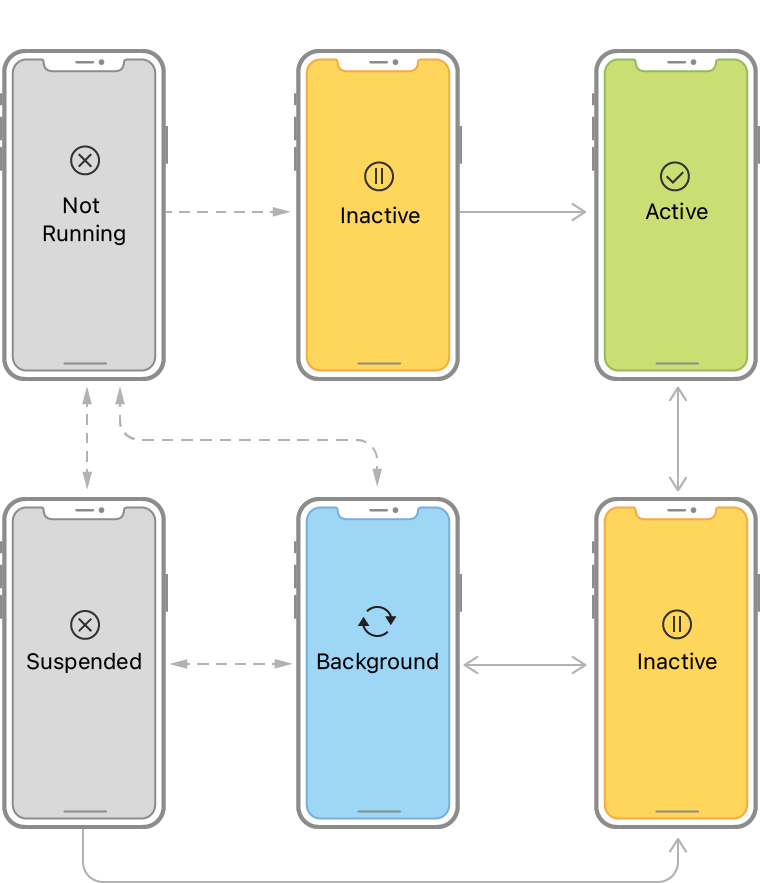
\includegraphics[width=10cm]{image2}
\caption{Lifecyle of iOS application}
\label{fig:image2}
\end{figure}

The picture shows that the application does not work at the beginning. At startup, the main window is inactive and the application has time to load the necessary data. Due to the imprecise name of the state, it should be noted that the inactive application is actually still running in the foreground, but is not receiving any events. After loading the data, the application is presented to the user, and events are sent to it. From this state, however, it can go into the background at any time, but it must go through the inactive state again. In the background, the application is then expected not to work or, with certain exceptions, to work only minimally. Another possible state is suspended, which the application enters when its code cannot be executed.

\subsubsection{Directly supported application architectures}
Apple Inc. directly supports the two architectures Model-View-Controller (MVC) and Model-View-ViewModel (MVVM) within Swift. In general, it is about dividing the system into three parts. The first is a framework that takes care of data storage and transformation. The second part is something that displays the data. In addition, the second part takes care of individual user inputs to the system. The last part is a kind of bridge between the first two parts.

MVC is one of the most widely used types of system architectures, so it has been supported in Swift since the beginning \footnote{\url{https://developer.apple.com/library/archive/documentation/General/Conceptual/DevPedia-CocoaCore/MVC.html}}. This support is provided by the UIKit library for iOS. However, in this architecture, programmers often created a controller that was too comprehensive and often disrupted the correct division of the application into modules. But in 2019 came the SwiftUI library, which brought direct support for MVVM. 
The difference is that there is no Controller. In this architecture, the user interface is described as the state of the application. Displayed windows are composed of instances of a structure that implements the View protocol. These structures create views. In order for the window to be dynamic, and therefore to be redrawable based on some event, we can give special attributes to individual views. These attributes use two-way binding (Binding) with the ViewModel or directly with the Model. Then we understand the state precisely as the sum of the values of the bound attributes. This state is always stored in the ViewModel object, which takes care of displaying windows and their views. To redraw the window, the state of the application must be changed, that is, at least one attribute linked to a view must be changed. It is necessary to point out that the entire window is not always redrawn, but only its views to which the changed states are linked.

\subsubsection{SwiftUI Framework}
The SwiftUI framework represents a protocol known as a view, which must be adapted by the structure in order to be displayed. The protocol requires the definition of the point attribute, whose value also implements the View protocol. Source code 3 shows the creation of a simple view that contains the text "Hello, World!" and a globe icon above it.

\FloatBarrier
\begin{kicode}{Swift}{} {HelloWorldView.swift}
struct HelloWorldView: View {
    var body: some View {
        VStack {
            Image(systemName: "globe")
                .font(.system(size: 100))
                
            Text("Hello World!")
                .font(.title)
                .padding(.bottom)
        }
        .padding()
    }
}
\end{kicode}
\FloatBarrier

\subsubsection{Handling view state}
Dynamics will be ensured by adding attributes that must be wrapped with a property wrapper (property wrapper, in the following text only the term wrapper is used) of a special type. A change in the wrapper values will then be propagated to the ViewModel, guaranteeing a redraw of the window. In his article [6], Paul Hudson explains the individual ways of tracking attribute changes.

The most important wrapper is \kiinlinecode{Swift}{!}{@State}, which can wrap attributes of simple data types and structures. Referenced types are observed using the \kiinlinecode{Swift}{!}{@ObservedObject} wrapper, which must implement the \texttt{ObservableObject} protocol. There is a \kiinlinecode{Swift}{!}{@Published} wrapper for marking tracked attributes in the referenced type. Referenced types can also be observed using the \kiinlinecode{Swift}{!}{@StateObject} wrapper, in which the application is responsible for the life cycle and not the user directly, as is the case with \kiinlinecode{Swift}{!}{@ObservedObject}. Another wrapper is \kiinlinecode{Swift}{!}{@EnviromentObject}, which allows you to get objects implementing the ObservableObject protocol that was created by views at a hierarchically higher level. Thanks to this, we do not have to sell these objects with arguments through several calls to views, which improves the overall readability of the code.

\subsubsection{Working with Views}
SwiftUI provides three basic window layout constructs \kiinlinecode{Swift}{!}{HStack}, \kiinlinecode{Swift}{!}{VStack}, and \kiinlinecode{Swift}{!}{ZStack}. They are used to store views next to each other based on a specified axis. \kiinlinecode{Swift}{!}{HStack} places views next to each other (from left to right),  \kiinlinecode{Swift}{!}{VStack} places them below each other (from top to bottom), and \kiinlinecode{Swift}{!}{ZStack} over them (from back to front).

Instead of the \kiinlinecode{Swift}{!}{Text} structure, we can insert points of other more complex structures into the body of the variable and thus create more complex windows and views. A \texttt{TextField} window is used to allow users to enter text. Using a parameter of type \kiinlinecode{Swift}{!}{Binding<String>}, this window can store input from the user in the variable provided by the parameter. A button represented by the Button structure is prepared for simple predefined user input. This structure requires two closures. The first defines what should happen when the button is pressed - the action and the second defines the content of the button.

Views can be formatted and their final appearance can be changed. For example, the \kiinlinecode{Swift}{!}{Text} structure can be formatted with methods that change the appearance of the text. Such a method is, for example, the \kiinlinecode{Swift}{!}{font} method changing the font size or \kiinlinecode{Swift}{!}{foregroundColor(Color)} changing the font color. The background color is changed using the background method. Changing the size of the view is possible with the \kiinlinecode{Swift}{!}{.frame} method.

\subsection{Server Application}
A server application has the task of mediating resources to one or, more often, to several users. While among the types of computer network structures, it is possible to find, for example, a client-server structure, which indicates the work of a server application. So it is a structure in which there is one main device (server), which is connected to the network and has some resources available. There are also other devices connected to the network that want to access the server's resources. These devices are referred to as client stations or clients. The server application waits for requests from clients. Server requirements vary based on what clients require. Requests can be sent, for example, using the HTTP protocol.

\subsubsection{HTTP Protocol}
The abbreviation HTTP comes from the English name of the protocol (Hypertext Transfer Protocol or in Slovakian Hypertext Transfer Protocol) used on the worldwide network (World Wide Web, abbreviated WWW). It works on the application layer described by the open systems interconnection model (the abbreviation OSI from the English translation The Open Systems Interconnection is used) \cite{bib1}. The protocol works on the transport protocol of controlled transmission (known as the abbreviation TCP from the English term Transmission Control Protocol).

Different types of HTTP requests have different semantics, but they may not be detailed enough for more complex servers. Therefore, servers tend to cluster work on some data. These clusters of data activities are then accessed using a uniform resource identifier (Uniform Resource Identifier or the more commonly used abbreviation URI), which is part of the URL in the HTTP request. The HTTP protocol uses nine types of requests, which are named methods. The most used, and thus the most frequently supported, methods are GET, POST, PUT, and DELETE. GET is a method used to get some data. The purpose of the POST method is to sell data to the server. PUT is used to replace some data. The DELETE request is intended to delete a document.
Each request must have a main header. Additional headers and their values are listed in the main header. The headers are, for example, the length of the body content (Content-length) or the authorized access header (Authorization), used for sending authorization code. The header can be followed by a body in which encoded data can be found.

\subsubsection{Programming of server applications}
When programming a server application, it is necessary to configure the server first. This configuration consists in creating and setting a kind of endpoint (the term socket is used in English), which connects the gateway (further on, only the English equivalent - port) of the device is used with the application. This configuration indicates to the operating system that the data sent to this device on this port is to be released to the application. The next step on the server side is to listen on that port. Listening means waiting until the operating system recognizes that a request has arrived for an application on a specified port. The operating system forwards the request to the application. The request should then be checked by the server and some work should be done. 

A frequently required practice is for the server application to always respond to the client with a message containing at least information on whether the request was processed correctly.
Although such a simple application will work correctly under certain circumstances, today's trend considers it incapable of normal functioning. If a new request arrives while the previous one is being processed, this request is ignored. To avoid dropping the right request due to load, requests can be stored in an array and processed sequentially. However, stored requests may not be processed quickly enough, so their time may run out. Therefore, processes and or threads are used. The application then has one main process that waits for requests in an infinite loop.

\begin{figure}[h!]
\centering
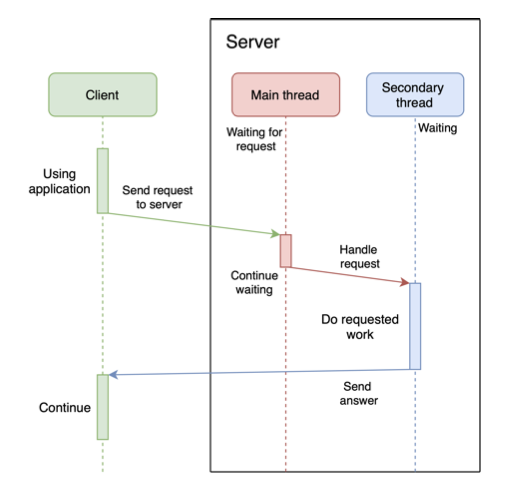
\includegraphics[width=10cm]{image1}
\caption{Parallelisation of request handling}
\label{fig:image1}
\end{figure}

After receiving the request, the main process creates a new thread to handle the request and then continues to wait. The child thread processes the request, performs some operations, and sends the response back to the client. Figure \ref{fig:image1} shows such a parallel reception of a request. The programmer then creates routes for individual supported request types and their possible variants or subsets. Paths have an identifier and some functionality. Thanks to the Identifier, it is possible to further divide the resources of the server application.

\subsection{Creating server applications using the Vapor framework}
The Vapor framework was created for creating server-side applications. It is a library with an expressive, protocol-oriented design focused on type safety. Vapor directly supports authentication using Basic or Bearer algorithms. It also supports working with database systems such as MySQL, PostgreSQL, SQLite, and MongoDB. It allows you to create HTML templates, it also allows you to create client and server applications using HTTP and many other concepts.

\subsubsection{Vapor basics}
Like any server application, an application created in the Vapor framework \cite{bib5} waits in an infinite loop for queries. To do this, Vapor uses concurrency, which allows an endless loop processing input and output processes. In order to ensure the processing of as many requests arriving at a similar time as possible, it is possible to operate processes from several threads. Working with processes is based on the modern Async/Await principle, which simplifies work with multiple threads and asynchronous processes.
This principle works in such a way that an asynchronous process is executed on another thread, while an object representing the result of the asynchronous code obtained sometime in the future is created in the current thread. It is possible to call other functions above this object and thereby determine further processing of the asynchronous result.

\subsubsection{Request routing}
Routing in this context is creating paths. Identifiers (parts of the path separated by the / symbol) and assigned functionality are assigned to paths. In the Vapor framework, this is done by registering individual paths. Registration consists of specifying the HTTP method, specifying the identifier, and defining the function itself.
There is an instance of the Application class and thus represents a server application. Using its get method, a block of code is defined for handling HTTP messages of type GET with the path HelloWorld. The method allows the creation of more complex paths using a variable number of arguments. The last argument is the closure, whose parameter is an object of type Request. This object represents the received HTTP request. The closure must return a value of a type that implements the Content protocol, and thus the returned type can be represented as an HTTP response. The return value is then serialized and sent as a response to the HTTP request.

\subsubsection{Creating a database}
To access the database, it is necessary to set the configuration, this consists of entering login data, the name of the database, and its location. Using this configuration, Vapor then takes care of connecting to the database. Vapor allows you to define and create database elements such as tables or initial data using migrations. The task of migration is to create or modify the table so that it appropriately represents the desired objects. Source Code 4 shows the migration to create and revert the SomeModelTable table. In the statement, the name of the table is successively set, then two columns are created, and finally, the entire table is created. Reverting a database is also a part of every model migration.

\FloatBarrier
\begin{kicode}{Swift}{}{Table creation using Vapor}
extension SomeModel {
    struct Migration: AsyncMigration {
        
        func prepare(on database: any Database) async throws {
            try await database.schema(schema)
                .id()
                .field(FieldKeys.name, .string, .required)
                .create()
        }
        
        func revert(on database: any Database) async throws {
            try await database.schema(schema)
                .delete()
        }
    }
}
\end{kicode}
\FloatBarrier

\subsubsection{Model representation}
A model \cite{bib6} that represents a single record and its relationships is used to access the individual rows of the table. Source code 5 shows a simple model for a someModelTable that has two columns: id and name. SomeModel is a final class that adapts the Model and Content protocols. By defining the schema variable, the class determines to which table the instances of the class will belong. The id variable is wrapped with the \texttt{@ID} wrapper, which indicates the private key. The second variable is wrapped by the \texttt{Field} wrapper, which has the task of representing an ordinary table column. Structure \texttt{FieldKeys} contains column names.

\FloatBarrier
\begin{kicode}{Swift}{}{Model representing in Vapor}
final class SomeModel: Model {
    
    static let schema: String = SchemaEnum.someModel.rawValue
    
    @ID
    var id: UUID?
    
    @Field(key: FieldKeys.name)
    var name: String
}
extension SomeModel {
    struct FieldKeys {
        static var name: FieldKey {"name"}
    }
}
\end{kicode}
\FloatBarrier

\subsubsection{Working with the database}
Vapor offers methods for working with the database directly in the Model protocol. The methods serve to create a database request and return the QueryBuilder type. Records can be filtered using the filter function, which takes as a parameter a predicate that the returned records must meet. The processing of the database request is processed asynchronously. The resulting records from the database can be obtained, for example, using the first (first record) or all (all records) methods.

\section{Analysis}
In this chapter, I analyze existing solutions, define requirements, outline use cases, and examine the integration of the iOS application with API.

\subsection{Existing solutions}
\subsubsection{Todoist}
Todoist is a popular task management application known for its simplicity and powerful features. It allows users to create tasks, organize them into projects and labels, set due dates and priorities, and collaborate with others. Main functionalities:
\begin{itemize}
	\item Task creation and organization
	\item Prioritization with labels and priority levels
	\item Due dates and reminders
	\item Collaboration features for sharing tasks and projects
	\item Integration with calendars, emails, and other applications
\end{itemize}

\subsubsection{Trello}
Trello is a flexible and visual task management tool based on the concept of Kanban boards. It allows users to create boards, lists, and cards to organize tasks and projects in a highly customizable way. Main functionalities:
\begin{itemize}
	\item Kanban-style task boards for organizing tasks into lists
	\item Drag-and-drop functionality for easy task management
	\item Customizable task cards with labels, due dates, and 
	\item Collaboration features for team 
	\item Integration with third-party tools and services
 \end{itemize}

\subsubsection{Jira}
Jira is a widely used project management tool developed by Atlassian. It is designed for agile teams and offers features for planning, tracking, and releasing software projects. Main Functionalities:
\begin{itemize}
	\item Agile project management with Scrum and Kanban boards
	\item Issue tracking and workflow management
         \item Customizable dashboards and reports
	\item Integration with development tools such as Git, Bitbucket, and Jenkins
	\item Extensive plugin ecosystem for additional functionalities
\end{itemize}

\subsection{Requirements}
Requirements of iOS and server applications are based on the main functionalities of applications that I analyzed in the previous section. Some of the requirements are also based on simplicity of use, eliminating problems of corporation-aimed tools, and providing users native OS experience.

\subsubsection{Operating system}
The mobile application supports the operating system iOS 17.

\subsubsection{Frameworks}
The mobile application uses SwiftUI as a UI framework. The server application is written in Swift 5 using the Vapor framework.

\subsubsection{Server architecture}
The server application implements REST API and conforms to its design principles.

\subsubsection{Authorization}
Users are authorized through a Bearer token for all endpoints that require authorization.

\subsubsection{User interface}
The user interface is designed to be native and user-friendly. It utilizes best practices of native iOS development and is inspired by system iOS applications.

\subsection{Use cases}

There are two user roles in the application - student and teacher. The use case diagram Figure \ref{fig:image3} shows activities that they can do.

\begin{figure}[h!]
\centering
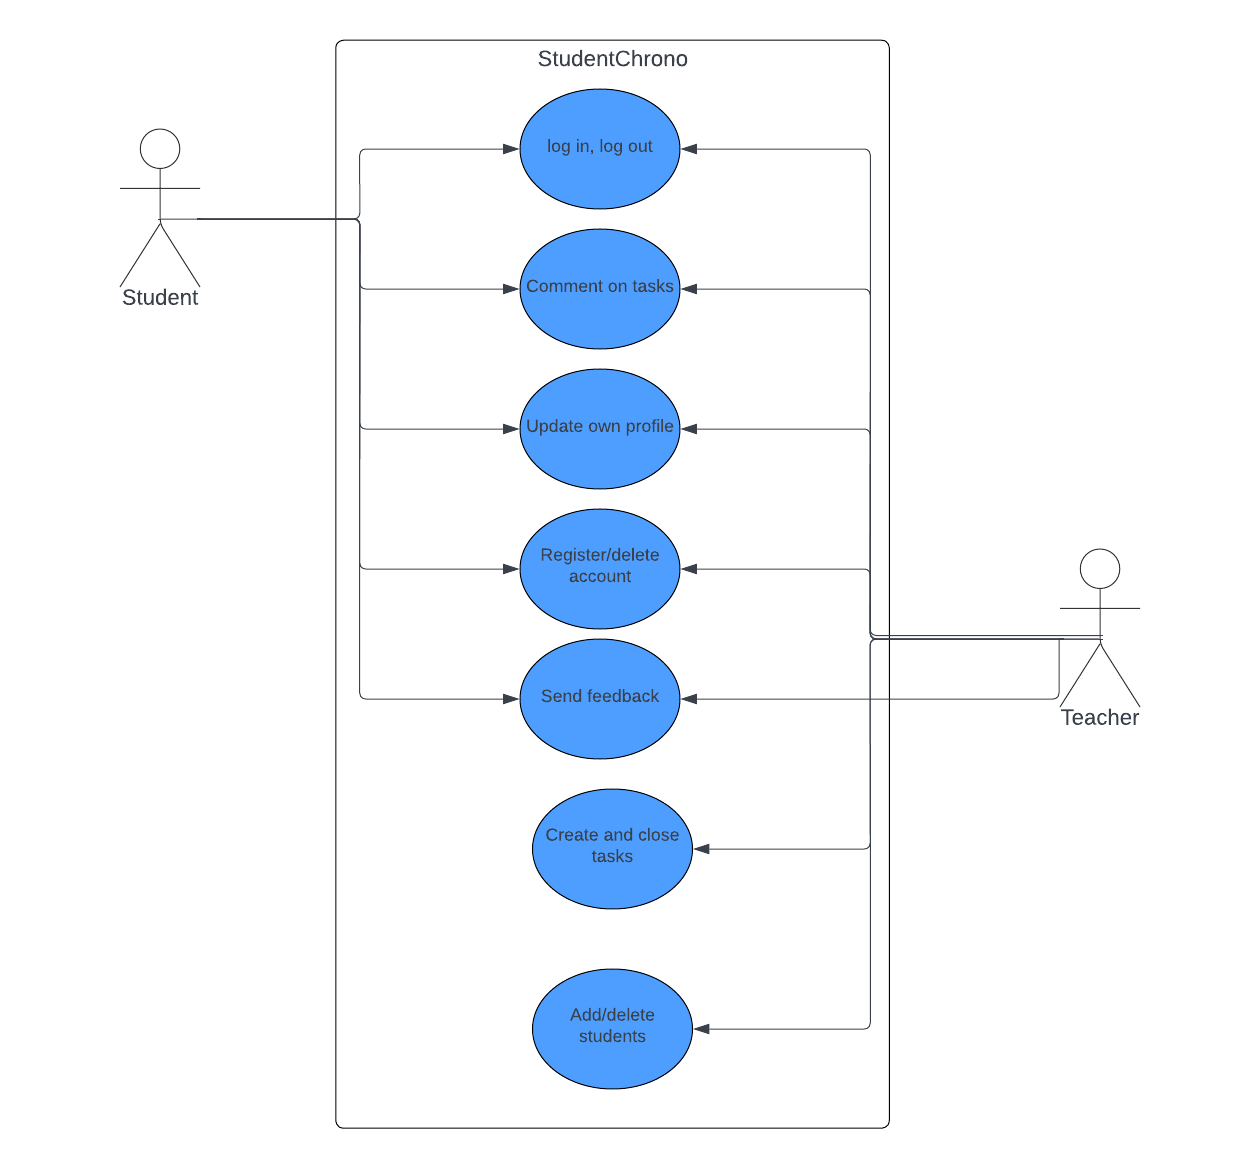
\includegraphics[width=15cm]{image3}
\caption{Use case diagram}
\label{fig:image3}
\end{figure}

\section{Mobile Application Design and Architecture}
In this chapter, I dive into the software and graphic design aspects of the applications. In the first part, I provide an overview of the design and architecture of the mobile application and the reasons for choosing it.
\subsection{Architecture}
I have chosen Clean Architecture \cite{bib7}, so the whole application is separated into three layers according to the Clean Architecture principles. Layers are Presentation, Domain, and Data Figure \ref{fig:image4} shows dependencies between layers. Further in the text, I will dive into the details of each layer.

\begin{figure}[h!]
\centering
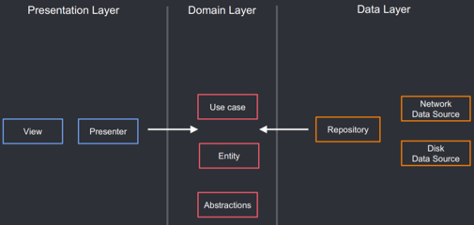
\includegraphics[width=15cm]{image4}
\caption{Depenencies in Clean Architecture}
\label{fig:image4}
\end{figure}

The mobile app utilizes advanced modularisation with SPM(Swift Package Manager) \cite{bib8}, so each layer is divided into logical parts. It also improves application build time, which is crucial during app development.

\subsubsection{Application Layer}
The application layer isn't a part of traditional Clean Architecture representation but is crucial for an application lifecycle. As displayed in Figure \ref{fig:image5} it contains:
\begin{itemize}
	\item Dependency Injection Package - helps to utilize dependency inversion and single responsibility principles by decoupling the usage of objects from its creations. Use cases, providers, and toolkits are registered there and then used in other parts of the application.
	\item Info folder - contains all \kiinlinecode{text}{!}{Info.plist} and other privacy files needed for application start.
	\item AppDelegate - object that manages the app's shared behaviors.
	\item AppFlowController, MainFlowController - top-level flow controllers of the application
\end{itemize}

These parts of the application are not suitable for the other layers, so they are in their own layer - Application.

\begin{figure}[h!]
\centering
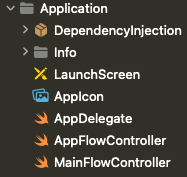
\includegraphics[width=8cm]{image5}
\caption{Application Layer}
\label{fig:image5}
\end{figure}

\subsubsection{Presentation Layer}
The presentation layer handles the user interface of the application. It is represented by FlowControllers and ViewModels + Views. This layer follows MVI architecture - each ViewModel has its state and intents, which are then used in a relevant SwiftUI View. Asynchronous functions are represented via native \kiinlinecode{Swift}{!}{async/await}.
Every app feature has its own presentation module (Onboarding / Tasks / Profile / Others) that contains Views + ViewModels. 

\subsubsubsection{FlowControllers}
Flow controllers control the flow of the app. All feature parts of the app should have their own flow controller, such as \kiinlinecode{Swift}{!}{OnboardingFlowController}, \kiinlinecode{Swift}{!}{AuthFlowController} etc. \kiinlinecode{Swift}{!}{AppFlowController} is the top-level flow controller, and it's defined in the Application layer. All flow controllers are a subclass of the \kiinlinecode{Swift}{!}{FlowController} class, which provides a common interface for all flow controllers. Flow controllers therefore inherit the \kiinlinecode{Swift}{!}{handleFlow()} method, which should be used in the view models to handle the flow. \kiinlinecode{Swift}{!}{handleFlow()} takes a parameter of type \kiinlinecode{Swift}{!}{Flow}, which is just an empty protocol, but all subflow enums (\kiinlinecode{Swift}{!}{OnboardingFlow}, \kiinlinecode{Swift}{!}{AuthFlow}, ...), which come with the feature flow controllers (\kiinlinecode{Swift}{!}{OnboardingFlowController}, \kiinlinecode{Swift}{!}{AuthFlowController}, ...), conform to this protocol, so that they can be used as the parameter of that method.

\FloatBarrier
\begin{kicode}{Swift}{}{Flow Example}
enum AuthFlow: Flow, Equatable {
    case auth(Auth)
    case login(Login)
    case registration(Registration)
    
    enum Auth: Equatable {
        case showLogin
        case showRegistration
    }
    
    enum Login: Equatable {
        case login(UserRoleEnum)
    }
    
    enum Registration: Equatable {
        case register
    }
}
\end{kicode}
\FloatBarrier

In this example, I then implement how the \kiinlinecode{Swift}{!}{ProfileFlowController} handles specific flows.

\FloatBarrier
\begin{kicode}{Swift}{}{Flow Handling Example}
override public func handleFlow(_ flow: 
	guard let authFlow = flow as? AuthFlow else { return }
        switch authFlow {
        case .auth(let authFlow): handleAuthFlow(authFlow)
        case .login(let loginFlow): handleLoginFlow(loginFlow)
        case .registration(let registrationFlow): handleRegistrationFlow(registrationFlow)
        }
}
\end{kicode}
\FloatBarrier

\subsubsubsection{Views and View Models}
Each top-level View has its own ViewModel, which handles the state of the entire view and passes data via \kiinlinecode{Swift}{!}{State} struct and \kiinlinecode{Swift}{!}{onIntent()} function handles interaction with View.

\FloatBarrier
\begin{kicode}{Swift}{}{ViewModel Example}
final class SomeViewModel: BaseViewModel, ViewModel, ObservableObject {

    // MARK: Dependencies
    private weak var flowController: FlowController?

    @Injected(\.someUseCase) private var someUseCase

    init(flowController: FlowController?) {
        self.flowController = flowController
        super.init()
    }

    // MARK: State
    struct State {
        var isLoading = false
        var items: [SomeDomainModel] = []
        var someInput = ""
        var alertData: AlertData?
    }

    @Published private(set) var state: State = State()

    // MARK: Intent
    enum Intent {
        case changeInput(to string: String)
        case cancel
    }

    func onIntent(_ intent: Intent)  {
        executeTask(Task {
            switch intent {
            case .changeInput(let string): changeInput(to: string)
            case .cancel: cancel()
            }
        })
    }

    private func changeInput(to string: String) {
        state.someInput = string
    }

    private func cancel() {
        flowController?.handleFlow(SomeFlow.flow(.dismiss))
    }
}
\end{kicode}
\FloatBarrier

The \kiinlinecode{Swift}{!}{executeTask()} function serves to handle tasks in each view model, so that all tasks will be cancelled when the view disappears.

\FloatBarrier
\begin{kicode}{Swift}{}{View Example}
struct SomeView: View {

    @ObservedObject private var viewModel: SomeViewModel

    init(viewModel: SomeViewModel) {
        self.viewModel = viewModel
    }

    var body: some View {
        SomeBackgroundView {
            VStack {
                SomeSubview(someInput: Binding<String>(
                    get: { viewModel.state.someInput },
                    set: { string in viewModel.onIntent(.changeInput(to: string)) }
                ))

                Button("Cancel") {
                    viewModel.onIntent(.cancel)
                }
            }
        }
    }
}
\end{kicode}
\FloatBarrier

\subsubsection{Domain Layer}
Domain layer reflects the whole business logic of the application via DomainModels and UseCases. It also defines protocols for repositories. This layer is separated into logical parts by feature.

\subsubsubsection{Domain models}
Domain models are used as the standard way to represent objects in the application. These models are used when passing data between layers
The app should only use these domain models and not models from some third-party libraries, as that would make the app strictly dependent on those specific libraries.  These models are defined under the Models directory for each logical part.

\FloatBarrier
\begin{kicode}{Swift}{}{Domain Model Example}
public struct AuthToken: Equatable, Codable {
    public let userId: String
    public let token: String
    
    public init(
        userId: String,
        token: String
    ) {
        self.userId = userId
        self.token = token
    }
}
\end{kicode}
\FloatBarrier

\subsubsubsection{Use Cases and their implementations}
Use cases represent the business logic functionalities. The presentation layer only calls these use cases, and that's where its responsibility ends. Use cases can call repository functions and other use cases. Each Use Case is represented by a protocol defining the \kiinlinecode{Swift}{!}{execute} function, allowing us to create more implementations, mocks, etc. Dependency Injection is then responsible for selecting the correct use case implementation. 

\FloatBarrier
\begin{kicode}{Swift}{}{UseCase example}
public protocol SomeUseCase {
    func execute() async throws
}

public struct SomeUseCaseImpl: SomeUseCase {
    
    private let repository: SomeRepository
    
    public init(repository: SomeRepository) {
        self.repository = repository
    }
    
    public func execute() async throws {
        try await someRepository.doSomething()
    }
}
\end{kicode}
\FloatBarrier

\subsubsubsection{Repositories}
Domain layer defines protocols for repositories - functions and their interfaces. Repositories are created for each logical part of the application.

\subsubsection{Data Layer}
The data layer is responsible for providing data via repositories and providers from the network. It is separated into \texttt{Toolkits} and \texttt{Providers}. There is a toolkit for each logical part of the domain layer. These toolkits provide repository implementations and relevant \texttt{NetworkModels}, \texttt{NetworkEndpoints}, etc. \texttt{Providers} define provider protocols and implementations.

\subsubsubsection{Repository implementation}
Repository implementations use providers and add some business logic. They're independent of the specific provider implementation. Repositories are registered for dependency injection in \texttt{DependencyInjection/Repositories.swift}

\FloatBarrier
\begin{kicode}{Swift}{}{Repository Implementation Example}
public struct SomeRepositoryImpl: SomeRepository {
    
    private let networkProvider: NetworkProvider
    
    public init(networkProvider: NetworkProvider) {
        self.networkProvider = networkProvider
    }
    
    public func someRepositoryMethod() async throws {
        try await networkProvider.request(SomeAPI.someEndpointNoParams)
    }
}
\end{kicode}
\FloatBarrier

\subsubsubsection{Providers implementation}
Providers are used for handling data sources. A provider is defined by protocol, each can have multiple implementations, for example, one using a third-party library, and another one using our own custom implementation. They also have to be registered for the dependency injection in \kiinlinecode{text}{!}{DependencyInjection/Providers.swift}

\FloatBarrier
\begin{kicode}{Swift}{}{Provider Example}
public protocol KeychainProvider {
    
    /// Try to read a value for the given key
    func read(_ key: KeychainCoding) throws -> String

    /// Create or update the given key with a given value
    func update(_ key: KeychainCoding, value: String) throws

    /// Delete value for the given key
    func delete(_ key: KeychainCoding) throws

    /// Delete all records
    func deleteAll() throws
}

public struct SystemKeychainProvider: KeychainProvider {
    public init() {}
    
    public func read(_ key: KeychainCoding) throws -> String {
        guard let bundleId = Bundle.app.bundleIdentifier else { throw KeychainProviderError.invalidBundleIdentifier }
        let keychain = Keychain(service: bundleId)
        guard let value = try? keychain.get(key.rawValue) else { throw KeychainProviderError.valueForKeyNotFound }
        return value
    }
    
    public func update(_ key: KeychainCoding, value: String) throws {
        guard let bundleId = Bundle.app.bundleIdentifier else { throw KeychainProviderError.invalidBundleIdentifier }
        let keychain = Keychain(service: bundleId)
        try keychain.set(value, key: key.rawValue)
    }
    
    public func delete(_ key: KeychainCoding) throws {
        guard let bundleId = Bundle.app.bundleIdentifier else { throw KeychainProviderError.invalidBundleIdentifier }
        let keychain = Keychain(service: bundleId)
        try keychain.remove(key.rawValue)
    }
    
    public func deleteAll() throws {
        for key in KeychainCoding.allCases {
            try delete(key)
        }
    }
}
\end{kicode}
\FloatBarrier

\subsection{Design}
In this section, I list the designed key components and their responsibilities.

\subsubsection{Screens}
Here I present the main Views of the iOS application. Each of them has a corresponding viewmodel.
\begin{itemize}
	\item \kiinlinecode{Swift}{!}{LoginView} and \kiinlinecode{Swift}{!}{RegistrationView}
	\item \kiinlinecode{Swift}{!}{TasksView}
	\item \kiinlinecode{Swift}{!}{CreateTaskView}
	\item \kiinlinecode{Swift}{!}{ProfileView}
\end{itemize}

\subsubsection{Server connection}
Below I list important data providing components with their description.
\begin{itemize}
	\item Models
	\begin{itemize}
		\item \texttt{User} - student or teacher;
		\item \texttt{Task}
		\item \texttt{AuthToken}
		\item \texttt{Message} - item of task elaboration
	\end{itemize}
	\item Repositories
	\begin{itemize}
		\item \kiinlinecode{Swift}{!}{AuthRepository}
		\item \kiinlinecode{Swift}{!}{UserRepository}
		\item \kiinlinecode{Swift}{!}{StudentsRepository}
		\item \kiinlinecode{Swift}{!}{TaskRepository}
		\item \kiinlinecode{Swift}{!}{FeedbackRepository}
	\end{itemize}
	\item Providers
	\begin{itemize}
		\item \kiinlinecode{Swift}{!}{NetworkProvider}
		\item \kiinlinecode{Swift}{!}{UserDefaultsProvider}
		\item \kiinlinecode{Swift}{!}{KeyChainProvider}
	\end{itemize}
\end{itemize}

\subsection{User Guide and Interface design}
In this chapter, I describe the application's UI and user's interacting with the application. User interface was designed based on native system look and Apple Human Interface Guidelines.

\subsubsection{Login and registration screen}
Users can register by providing their name, surname, birthday, and email or log in to the application through email and password. The application supports two roles - student and teacher. The role is selected during registration, only users older than 18 years can be teachers. Users can log out of the application and delete the account if needed.

\begin{figure}[h!]
\centering
\begin{minipage}[b]{0.4\textwidth}
	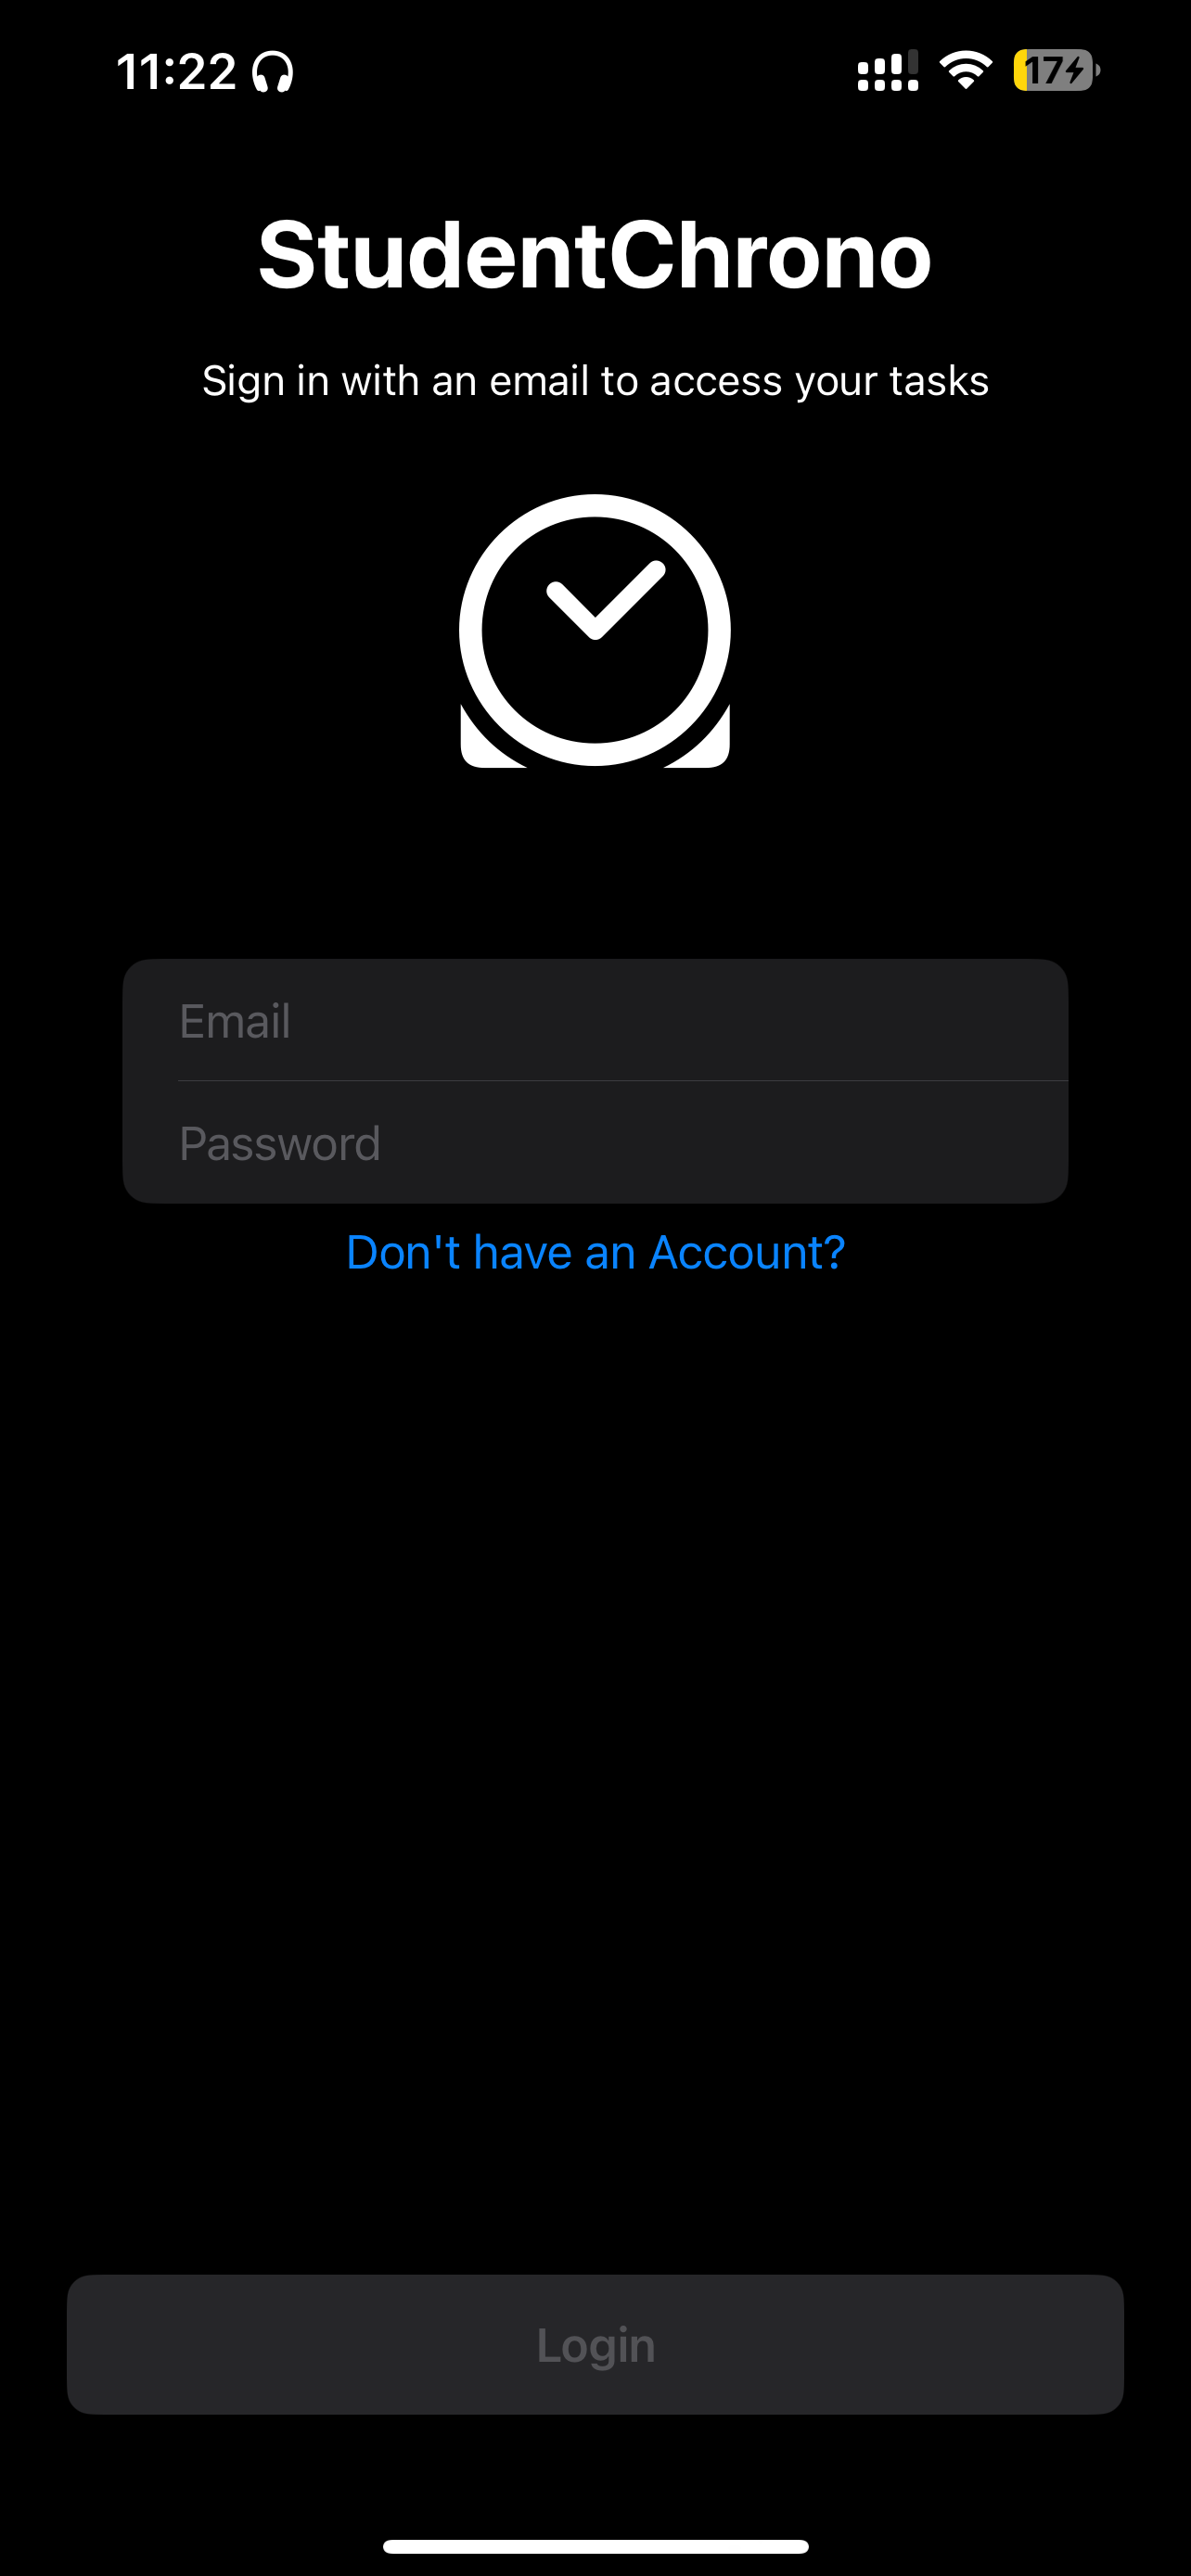
\includegraphics[height=10cm]{image6}
\end{minipage}
\begin{minipage}[b]{0.4\textwidth}
	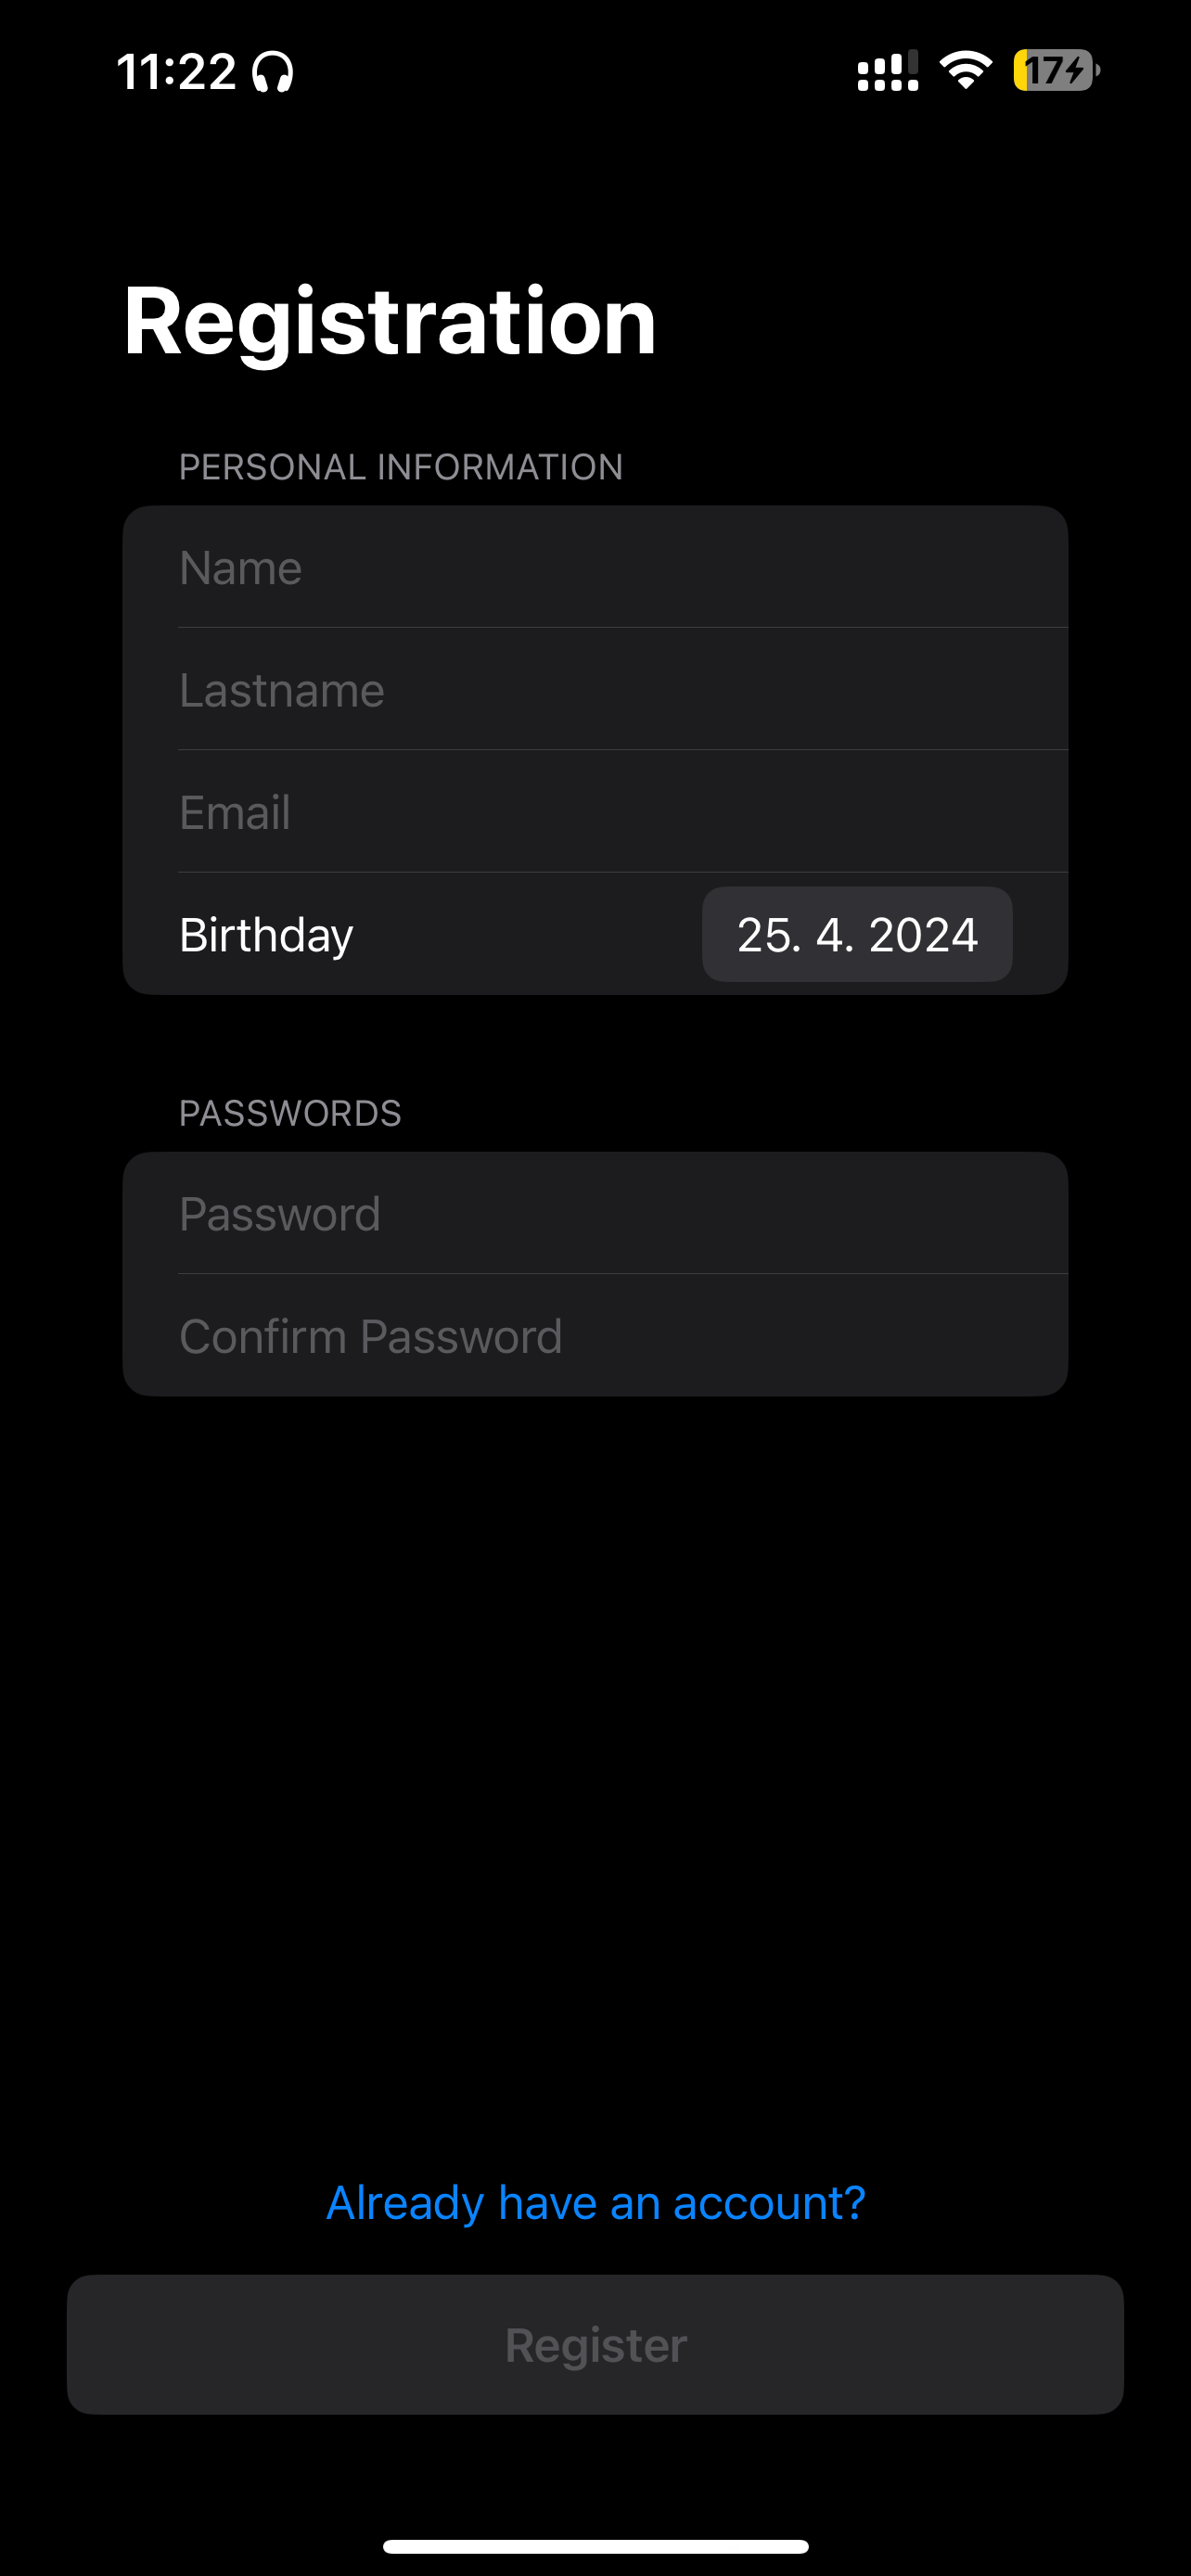
\includegraphics[height=10cm]{image7}
\end{minipage}
\caption{Login and registration views}
\label{fig:image6-7}
\end{figure}

\subsubsection{Tasks list and task detail screen}
Users with teacher roles can create tasks,  assign them to their students, see all the tasks they created, and control task elaboration. Users with student roles can see all the tasks they were assigned, their current status, author, and deadline. Users can provide comments and files for task elaboration in the form of comments.

\begin{figure}[h!]
\centering
\begin{minipage}[b]{0.4\textwidth}
	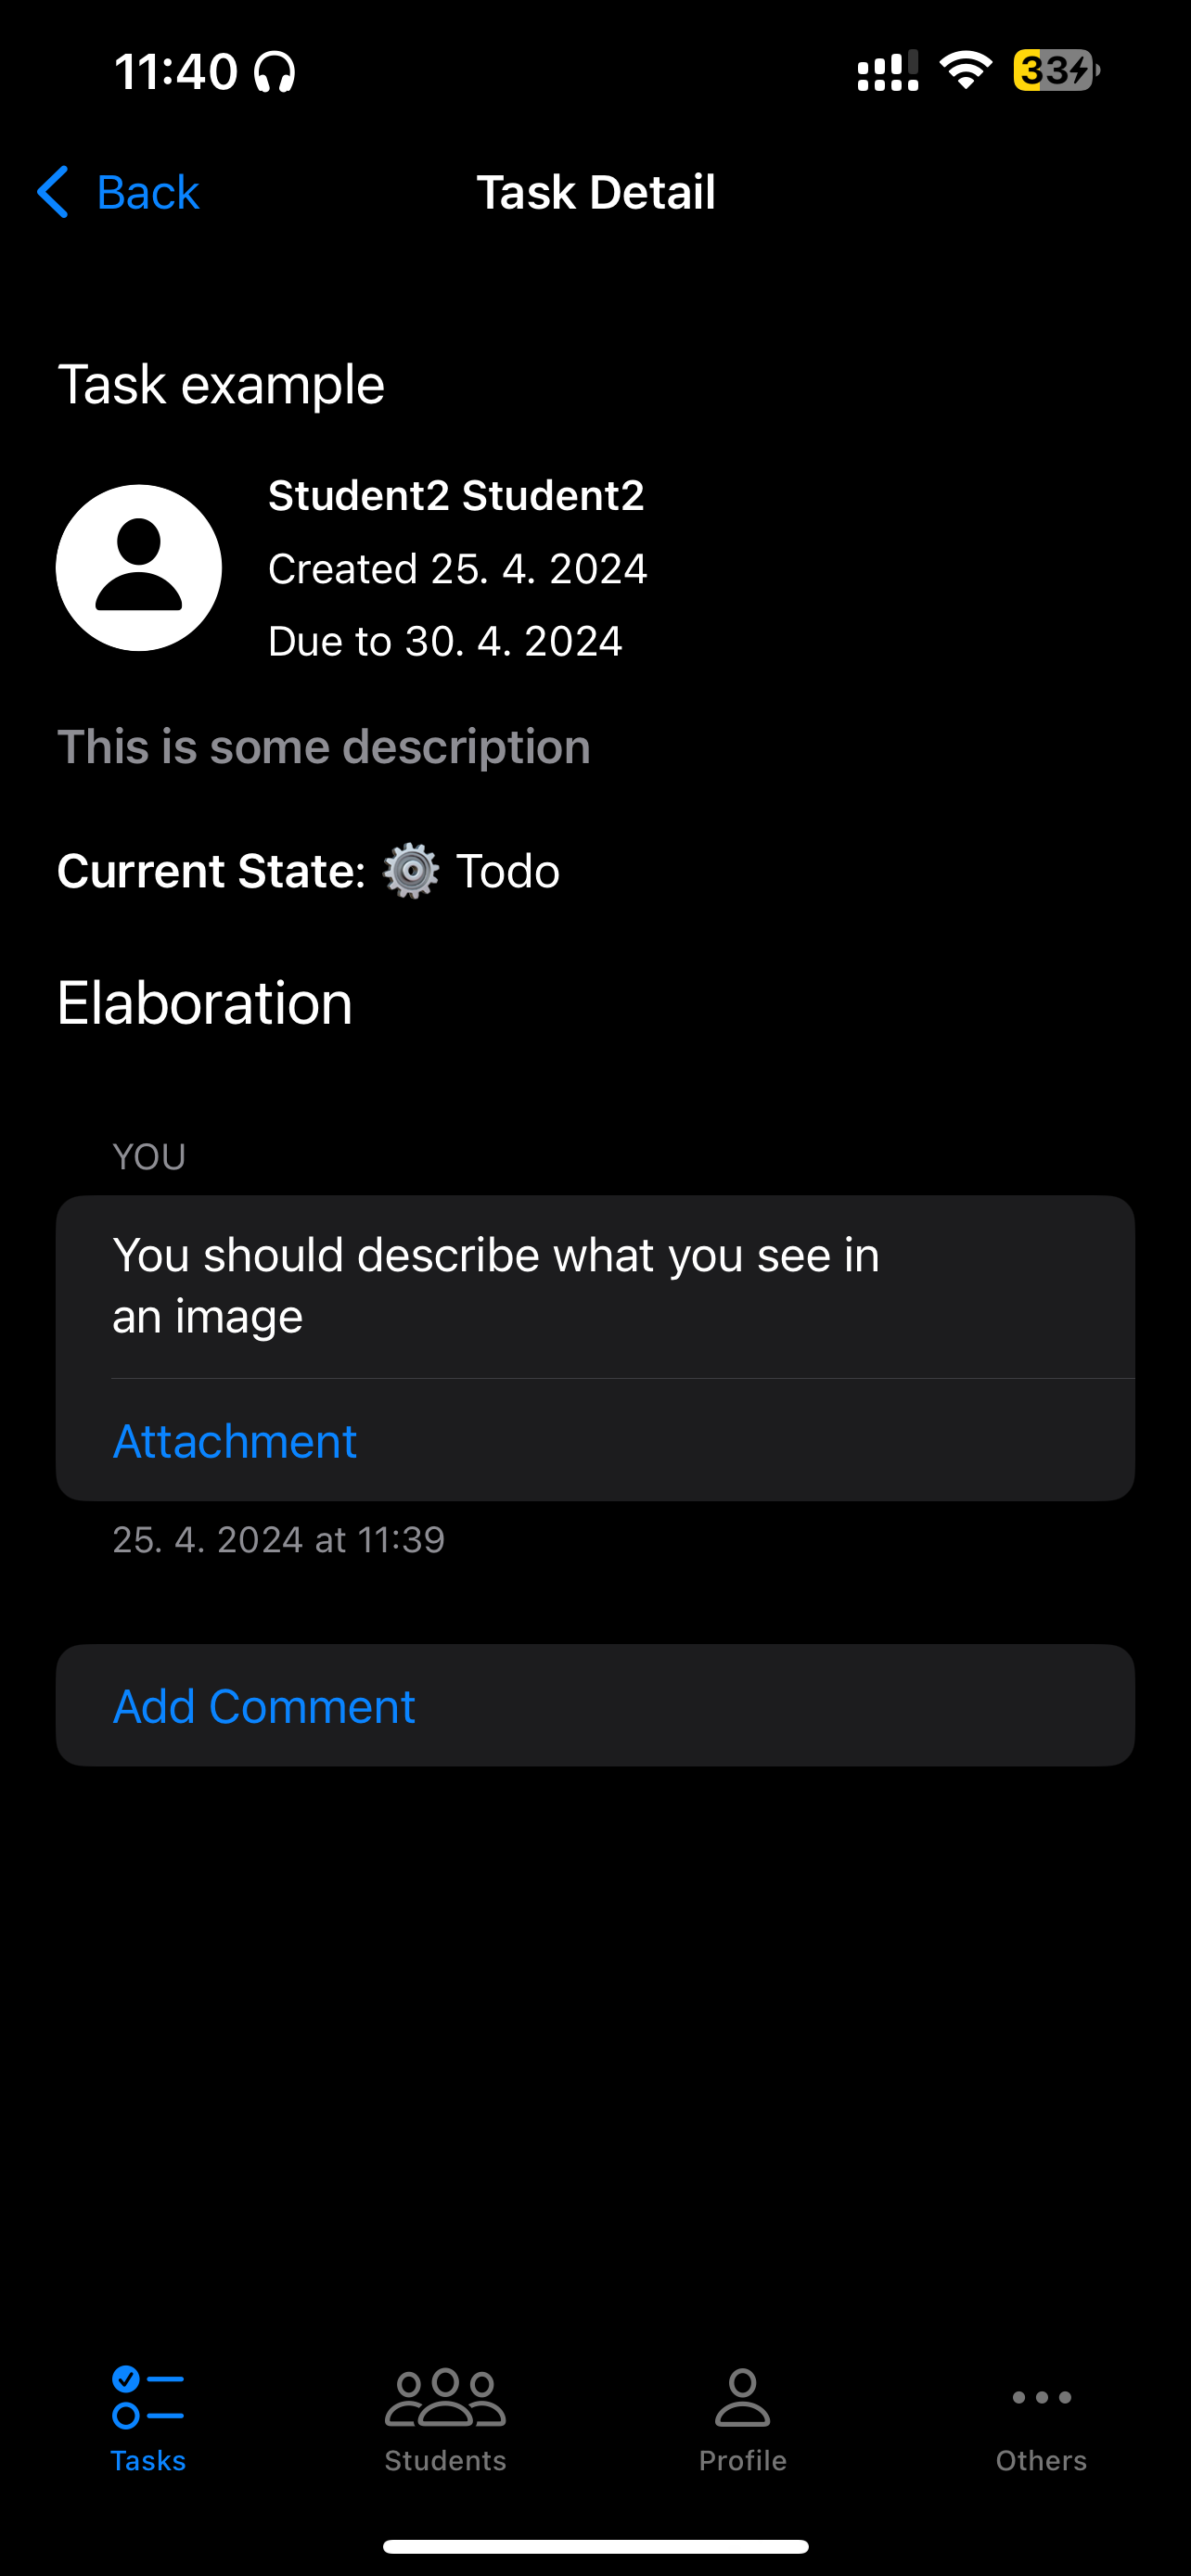
\includegraphics[height=10cm]{image8}
\end{minipage}
\begin{minipage}[b]{0.4\textwidth}
	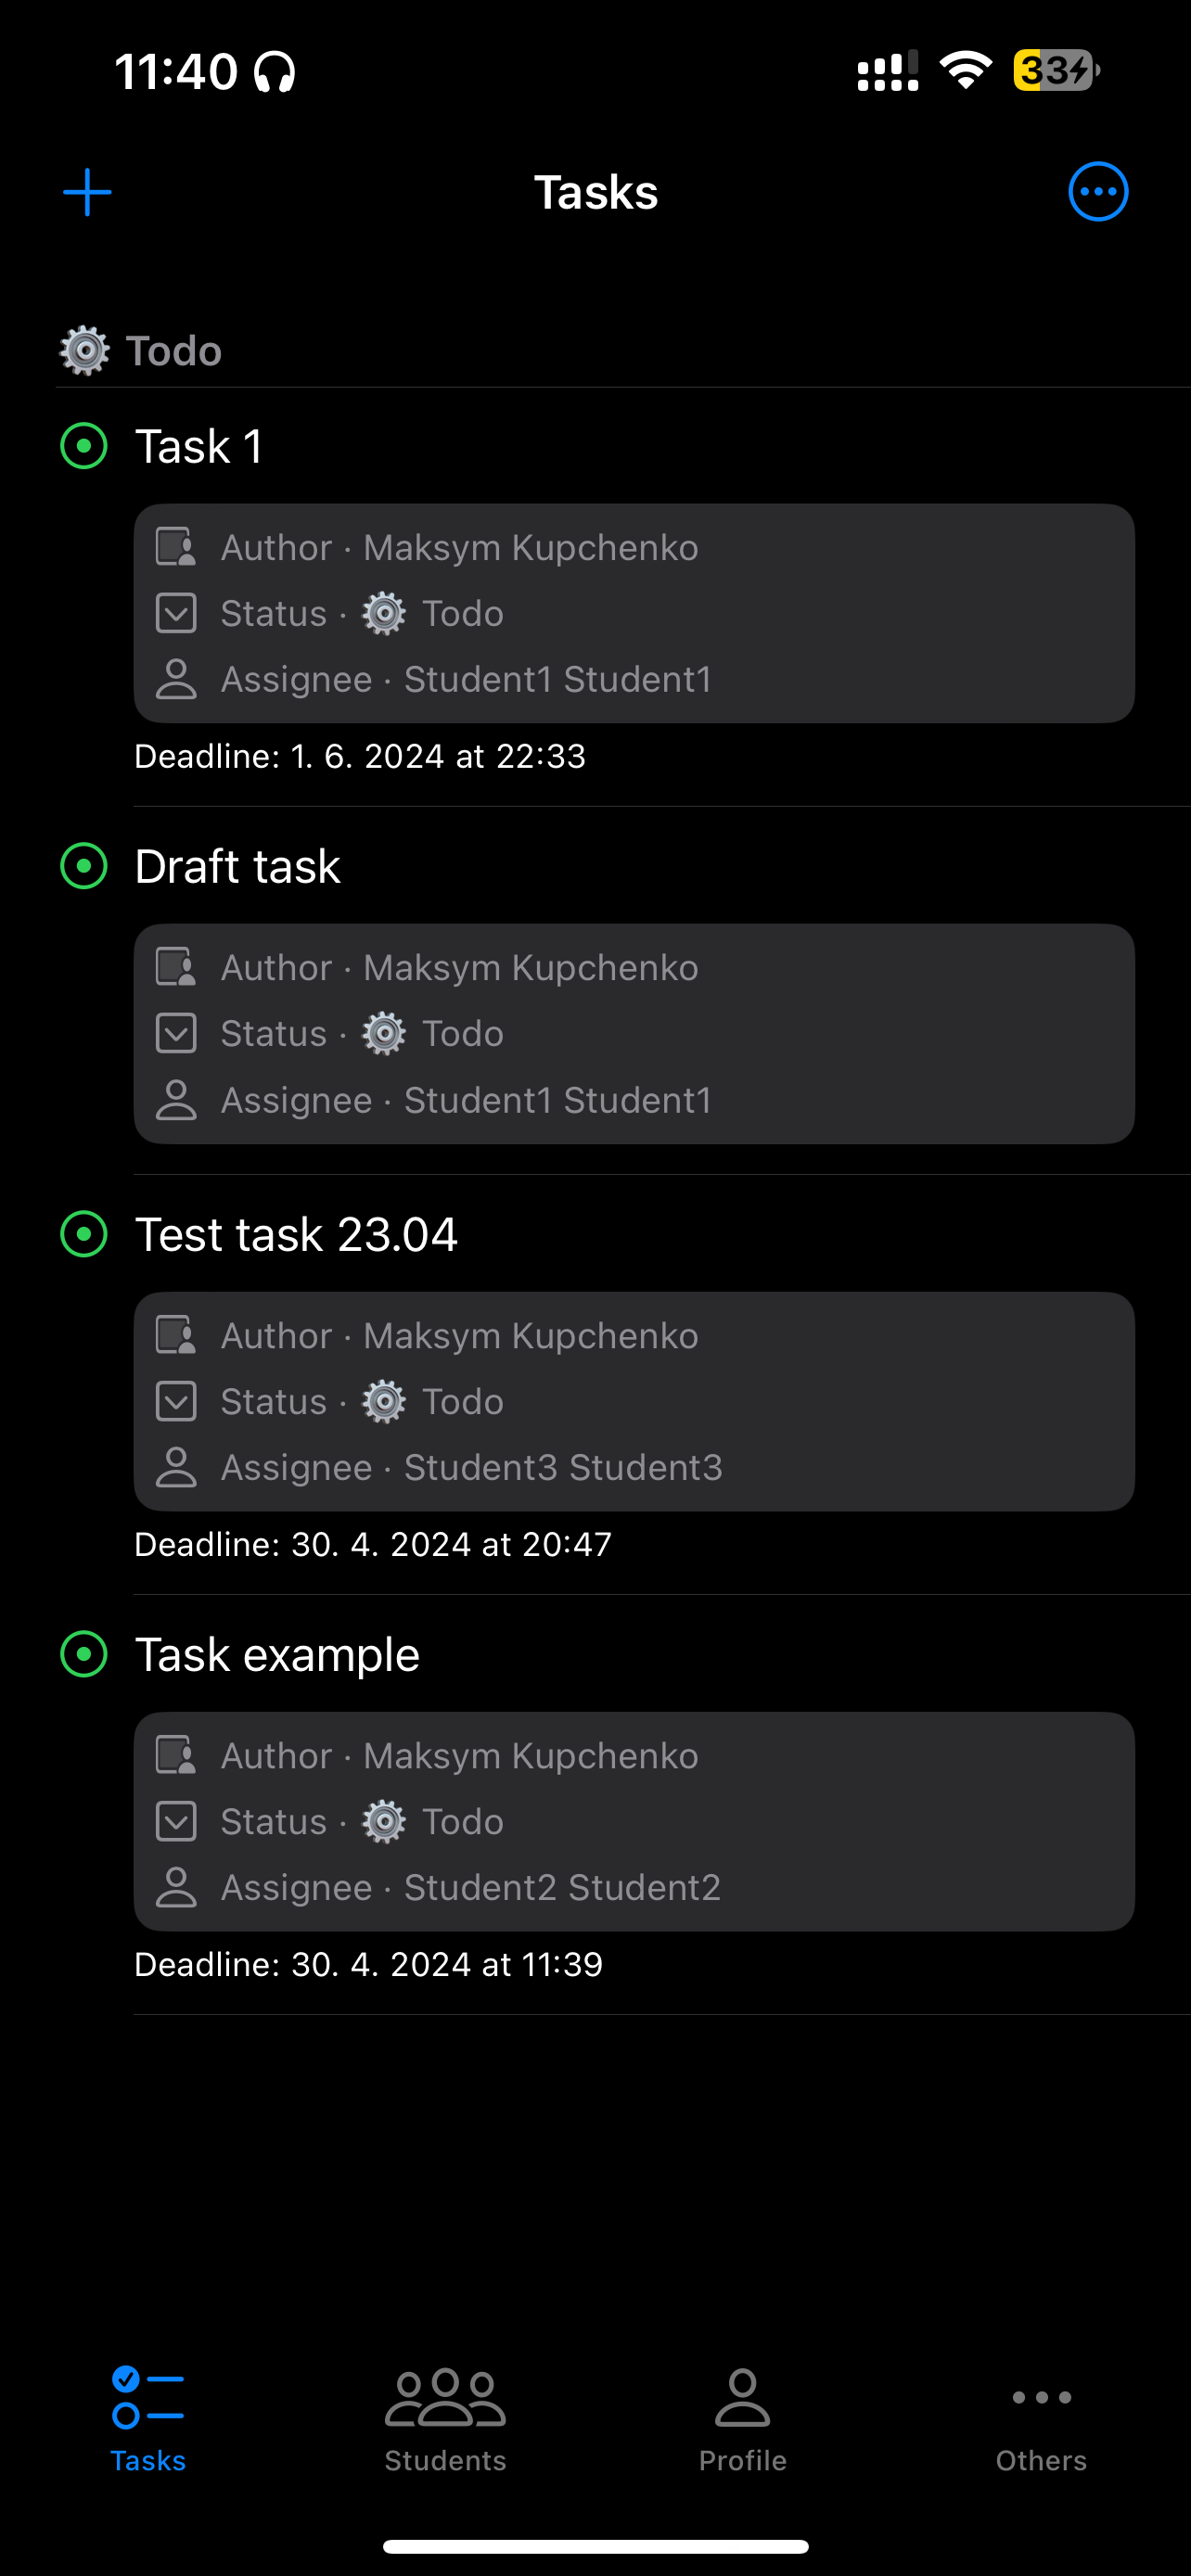
\includegraphics[height=10cm]{image9}
\end{minipage}
\caption{Task List and Task Detail}
\label{fig:image8-9}
\end{figure}

\subsubsection{Create task screen}
This is one of the key screens of the entire application. Here teachers can create tasks, provide a description, deadline, priority and assign them to students.

\begin{figure}[h!]
\centering
\begin{minipage}[b]{0.4\textwidth}
	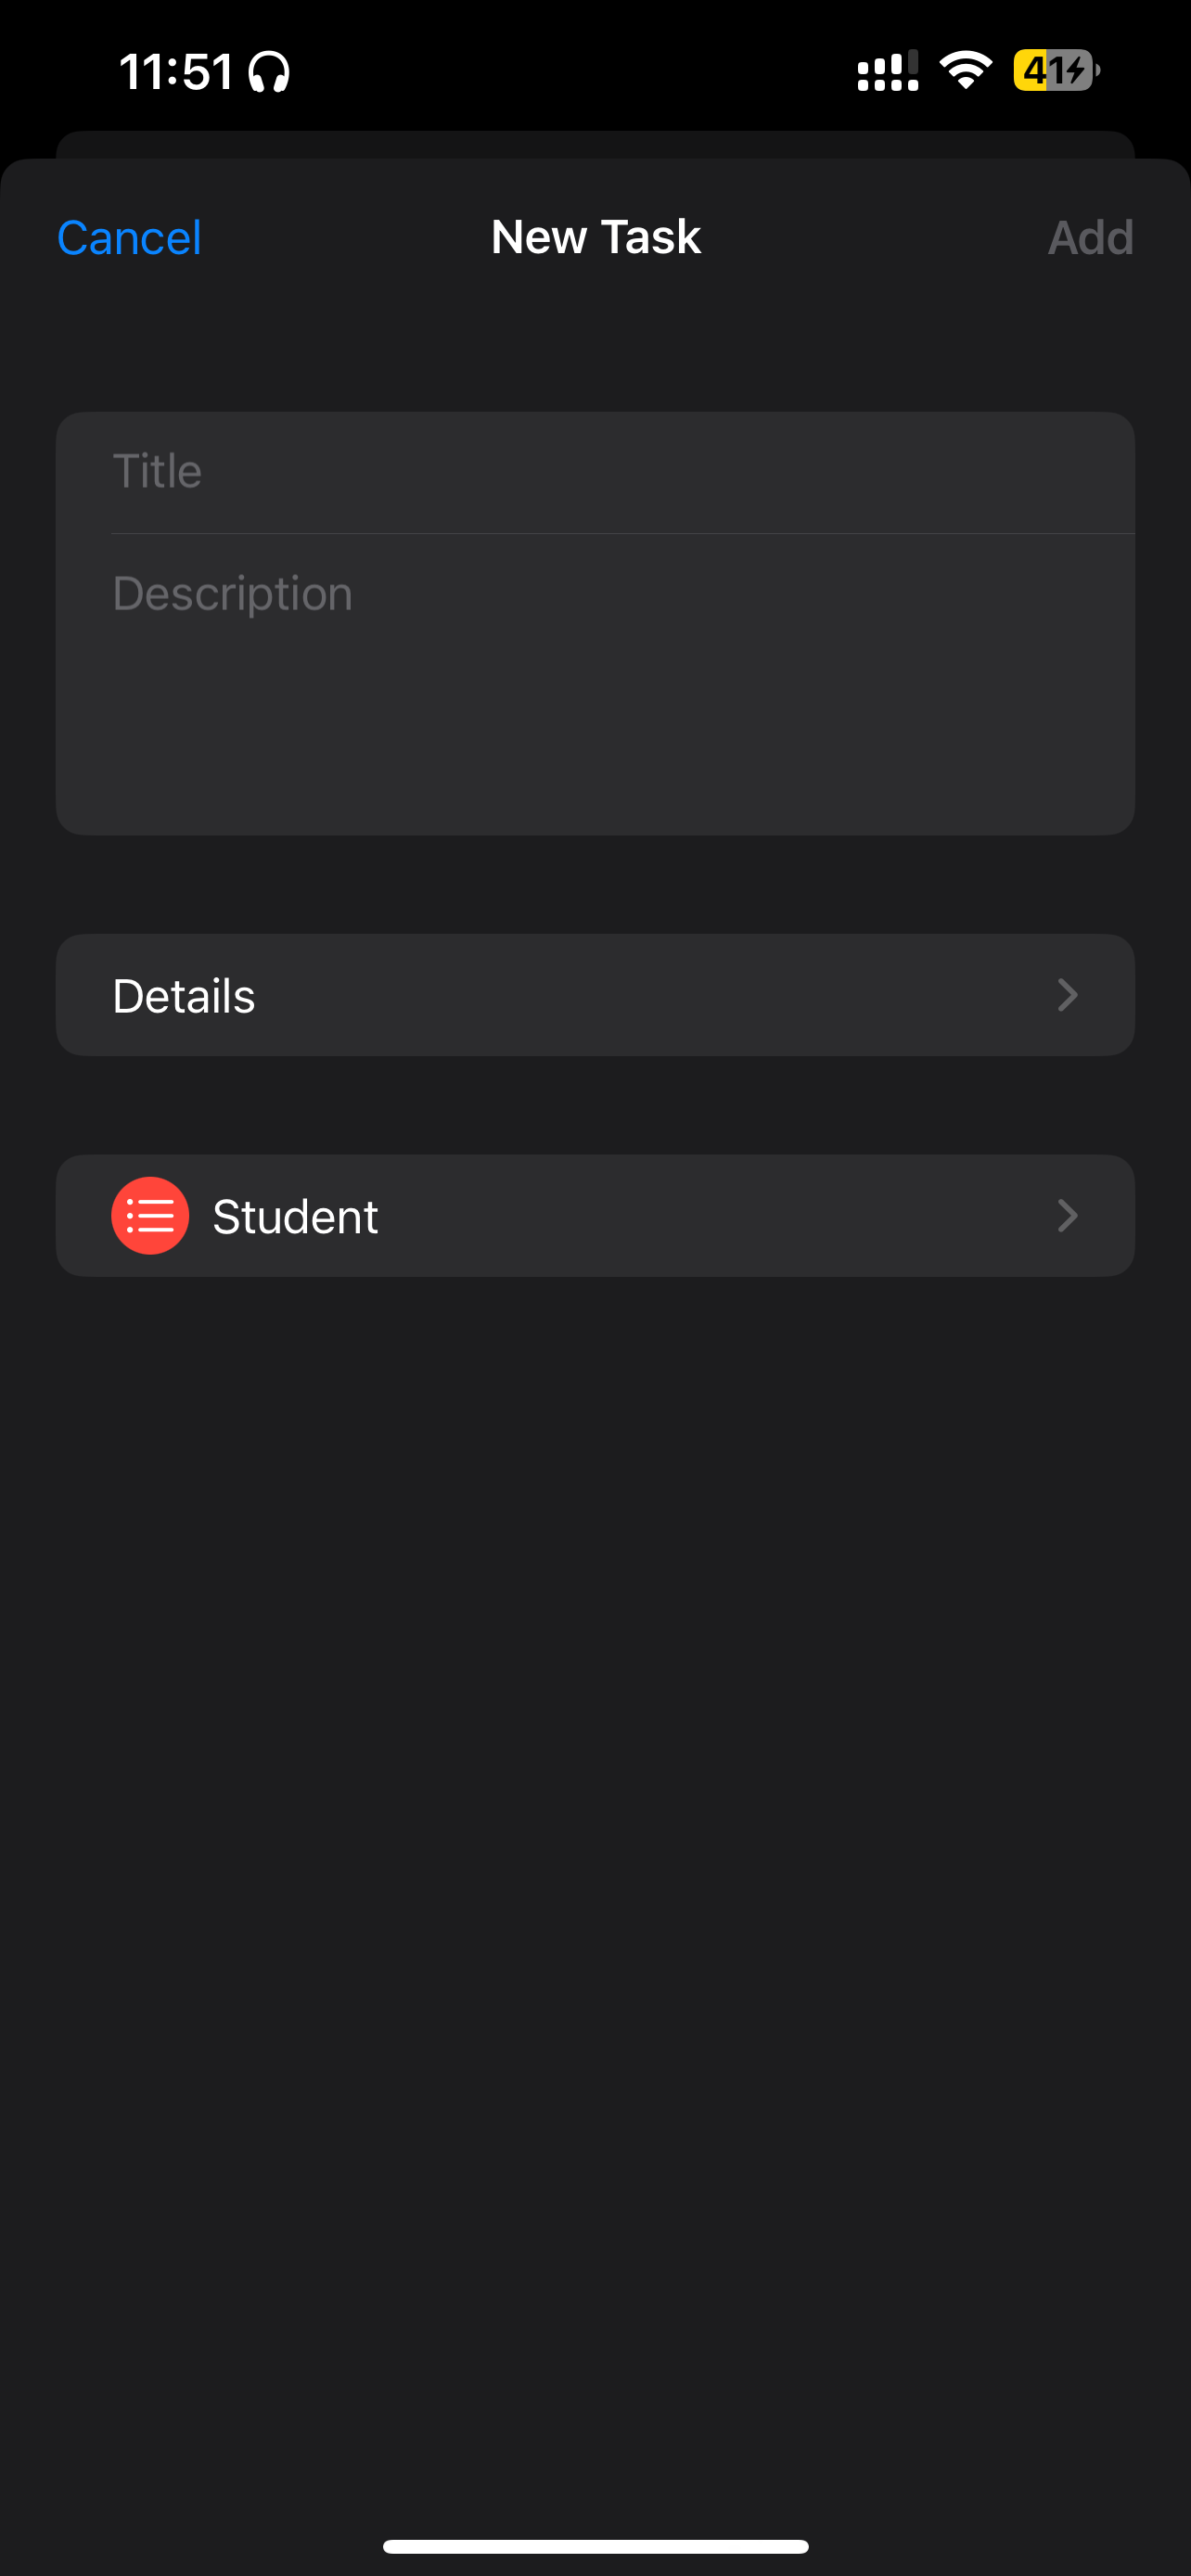
\includegraphics[height=10cm]{image10}
\end{minipage}
\begin{minipage}[b]{0.4\textwidth}
	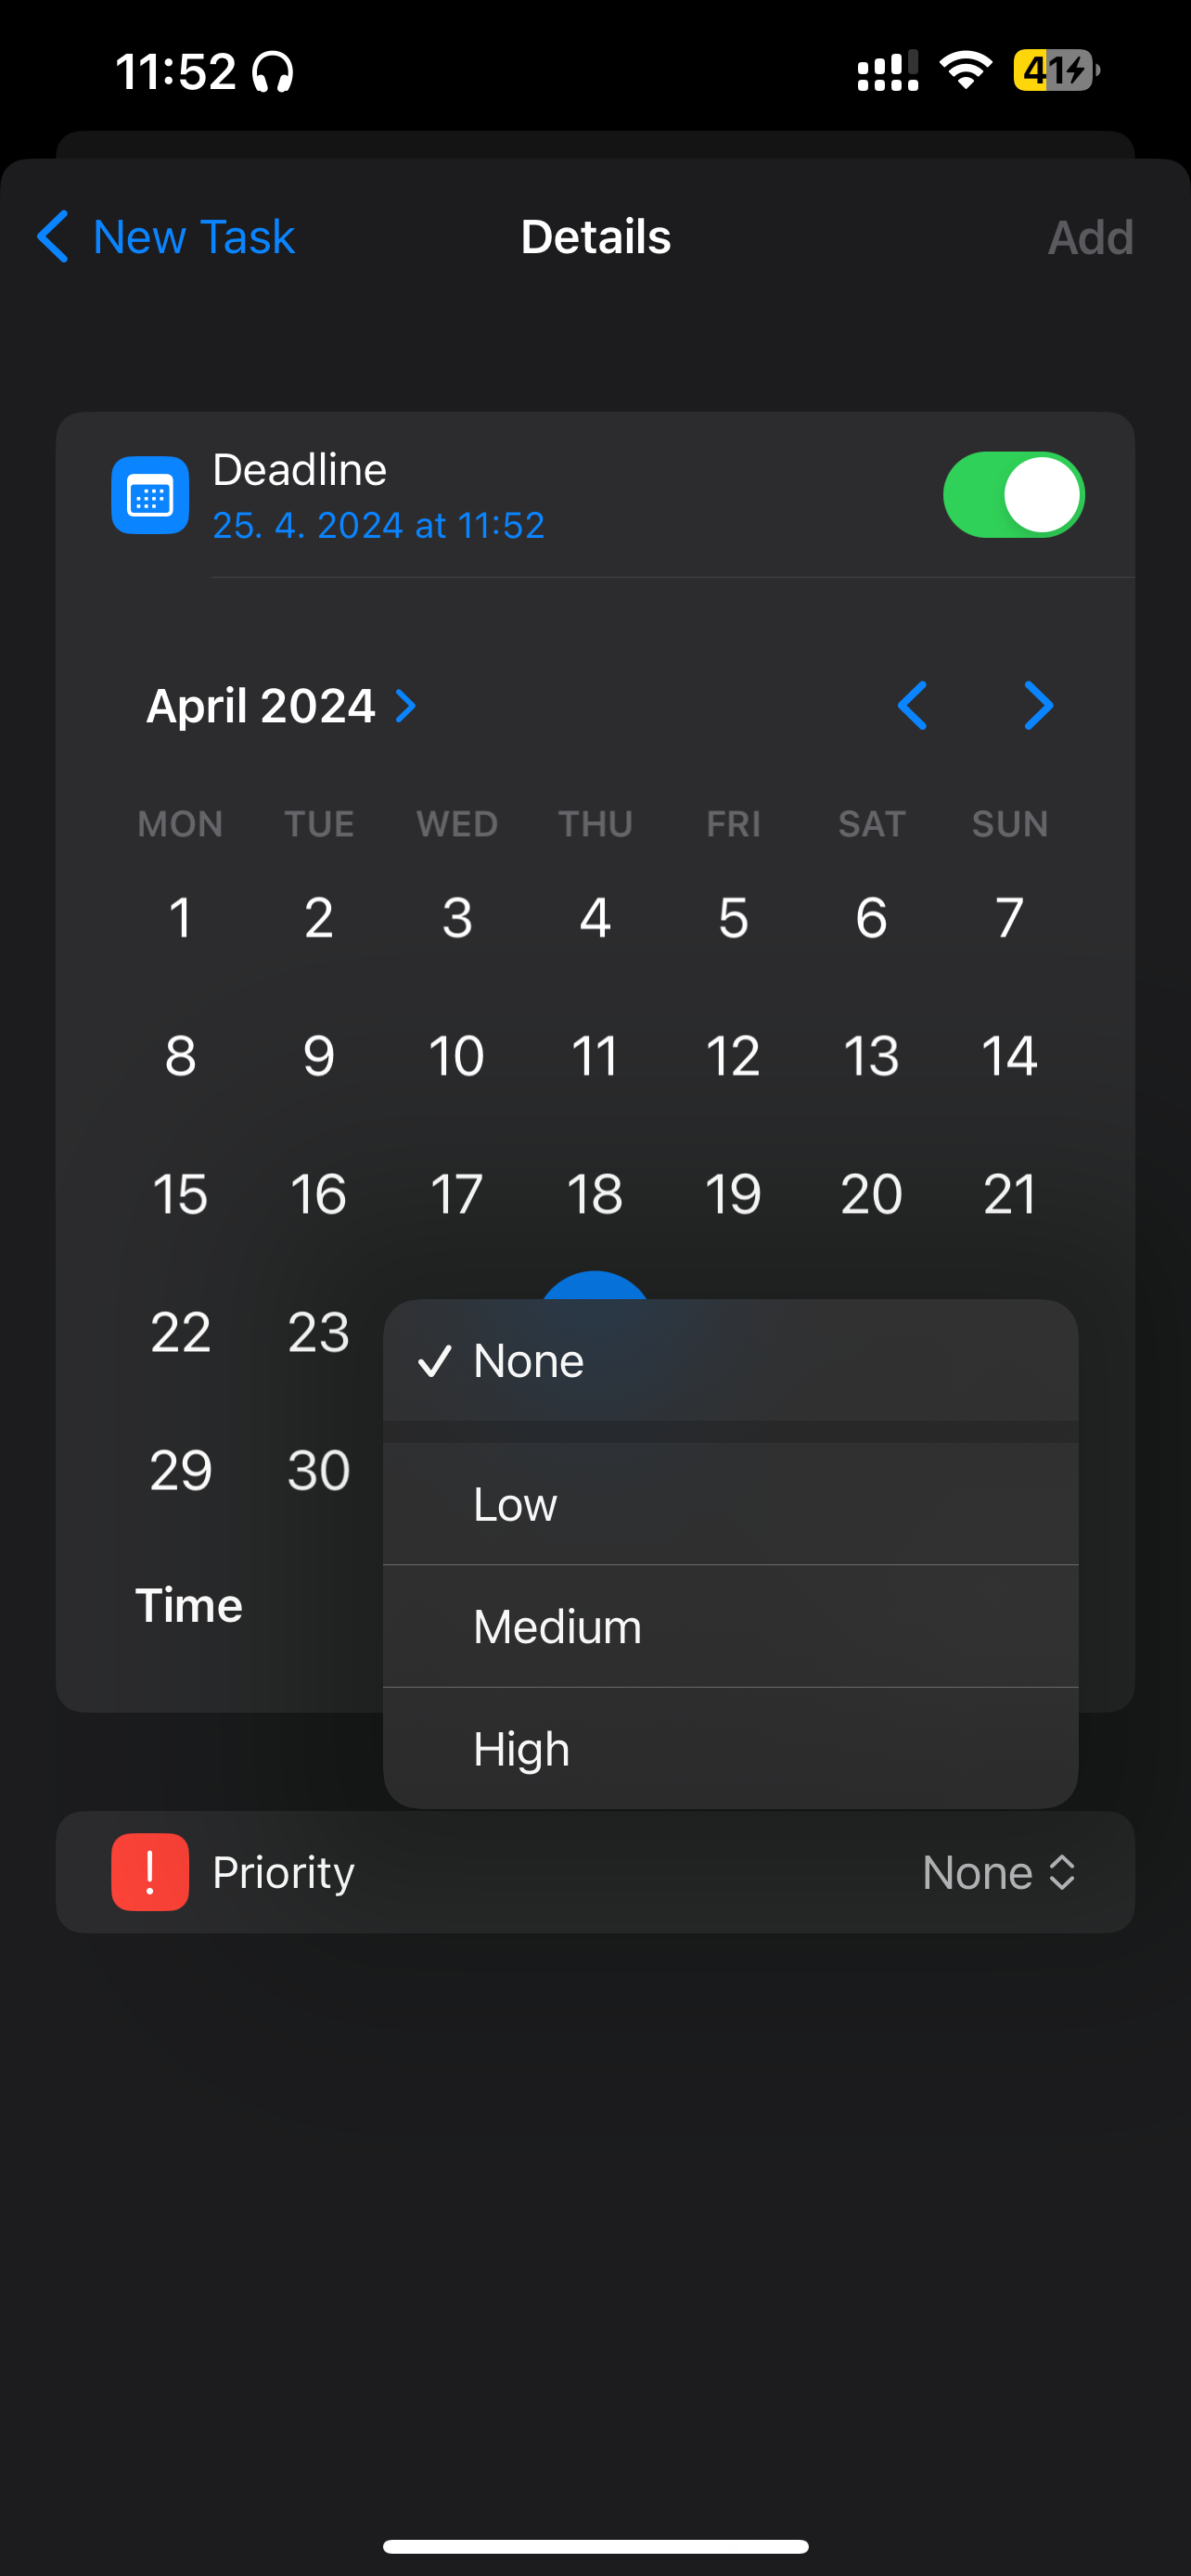
\includegraphics[height=10cm]{image11}
\end{minipage}
\caption{Create task screen}
\label{fig:image10-11}
\end{figure}

\subsubsection{Profile screen}
Here users can update their personal information, such as name and surname, upload profile photo and update their password if needed.
\begin{figure}[h!]
\centering
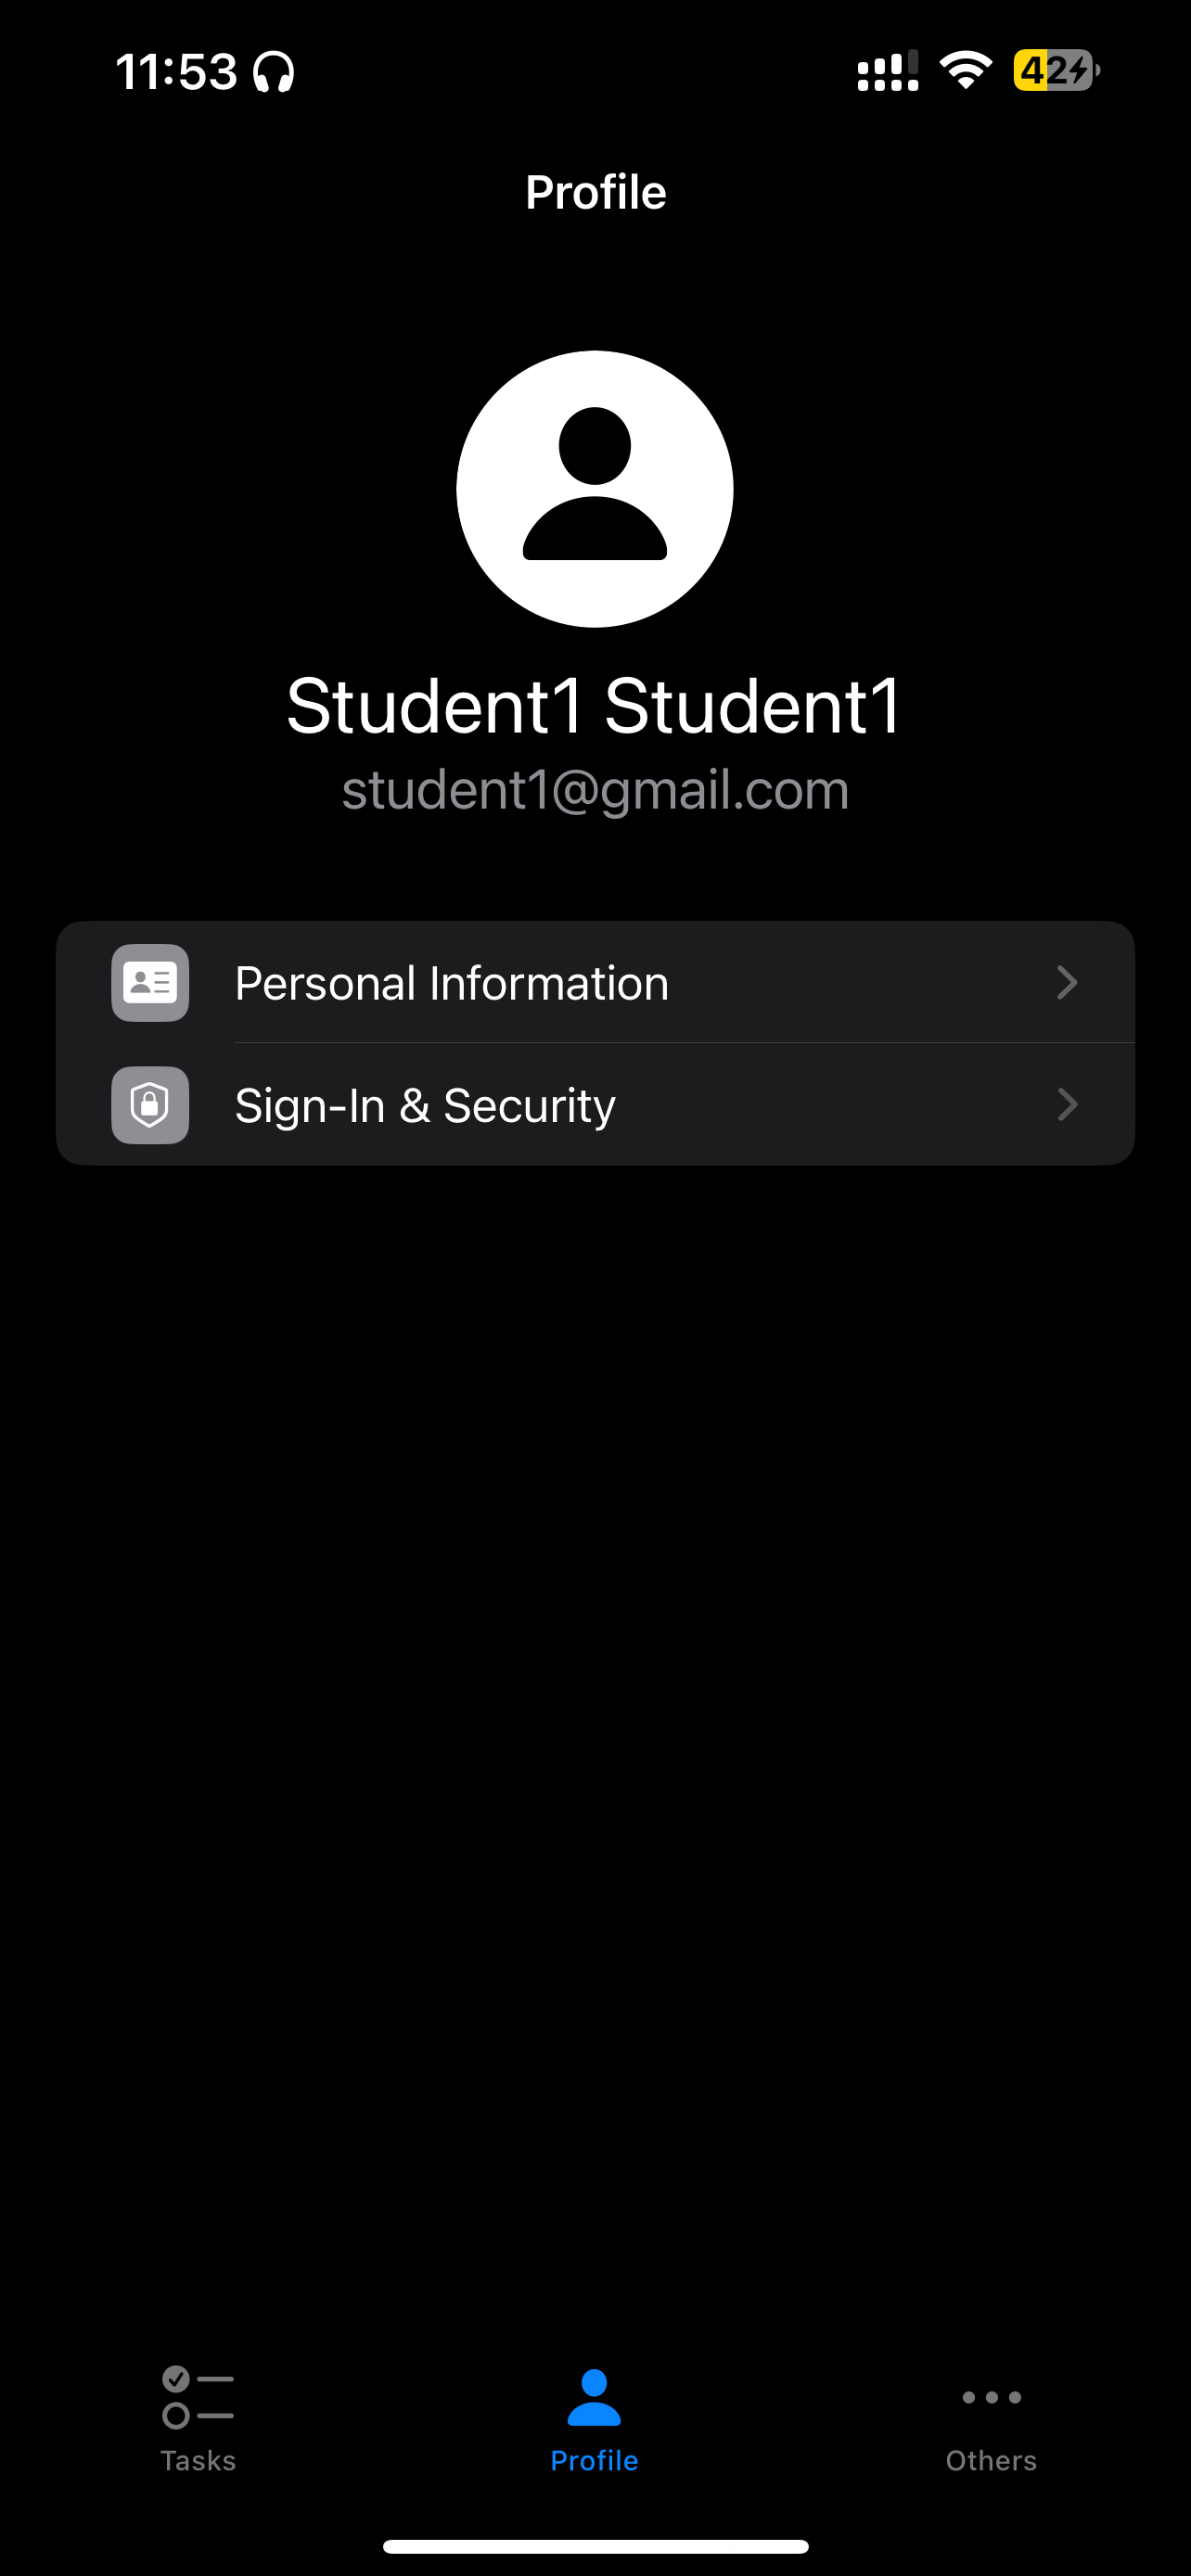
\includegraphics[height=10cm]{image12}
\caption{Profile Screen}
\label{fig:image12}
\end{figure}

\section{Server-side application design}
In this chapter, I dive into designing the architecture of the web application and explain my decisions.

\subsection{MVC architecture}
Server-side applications often use the Model-View-Controller (MVC) architectural pattern, which separates the application into three interconnected components:

\begin{itemize}
	\item \texttt{Model}  - represents the data and business logic of the application. It encapsulates the underlying data structures, performs data manipulation operations, and enforces business rules. In web applications, models typically correspond to database tables or external data sources and define the structure and behavior of the data.
	\item \texttt{View} - handles the presentation layer of the application, responsible for rendering data and generating responses to client requests. In API applications, views are often represented as JSON representations of the underlying data. Views in backend applications focus on serializing data into a format that can be easily consumed by clients.
	\item \texttt{Controller} - acts as an intermediary between the model and the view, handling incoming requests, processing data, and generating appropriate responses. They contain route handlers that define the behavior of different endpoints in the application. They parse incoming requests, invoke the appropriate business logic in the model layer, and format the response data for the client.
\end{itemize}

\subsection{Routing}
Routing is a fundamental aspect of server-side applications, defining how incoming requests are mapped to specific controller actions. Routes in API applications are typically configured using a routing table or configuration file, which maps URL patterns to corresponding controller actions. Routes specify the HTTP method (GET, POST, PUT, DELETE) and URL path for each endpoint, allowing to define the behavior of different API endpoints.

\subsection{Middleware}
Middleware are components that intercept incoming requests and outgoing responses, allowing adding any functionality to the request-response lifecycle. Common uses of middleware in API applications include authentication, authorization, request logging, error handling, and request validation. Middleware can be chained together to create a middleware pipeline, where each middleware component processes the request and passes it on to the next component in the pipeline.

\section{Implementation}
This chapter is about the implementation of the iOS and server-side applications which I implemented by architecture and design described in the earlier chapter. I point out some interesting implementation parts and decisions I made. The project with all source code can be found in the public GitHub repository\footnote{\url{https://github.com/maxkup19/bachelor-thesis}}.

\subsection{iOS application}
\subsubsection{User interface development}
Mobile application is created based on the design provided in previous parts using primarily SwiftUI framework. \texttt{Tasks screen} that is considered as the main application's screen is presented by \texttt{TasksView}. It consists of \texttt{TaskList} if tasks are present, and \kiinlinecode{Swift}{!}{ContentUnavailabelView} otherwise. The screen has the title "Tasks" and a button to create a new task if the user has a teacher role.

\FloatBarrier
\begin{kicode}{Swift}{H}{TasksView}
struct TasksView: View {
    @ObservedObject private var viewModel: TasksViewModel
    init(viewModel: TasksViewModel) {
        self.viewModel = viewModel
    }
    var body: some View {
        VStack {
            if !viewModel.state.isLoading && viewModel.state.tasks.isEmpty {
                ContentUnavailableView(
                    "No tasks",
                    systemImage: "list.bullet",
                    description: Text("You have no tasks available")
                )
            } else {
                TasksList(
                    tasks: viewModel.state.tasks,
                    onTaskTap: { id in viewModel.onIntent(.onTaskTap(id))},
                    onRefresh: { viewModel.onIntent(.refreshTasks) }
                )
            }
        }
        .navigationTitle("Tasks")
        .toolbar {
            ToolbarItem(placement: .topBarLeading) {
                if viewModel.state.showCreateButtonTask {
                    Button(action: { viewModel.onIntent(.createTask) }) {
                        AppTheme.Images.plus
                    }
                }
            }
        }
    }
}
\end{kicode}
\FloatBarrier

Other views also have same structure, subviews don't have their own viewmodels, but the data is passed from high-level viewmodels. through initializers.

ViewModels have a specific structure to conform to an MVI architecture, so it always has some \kiinlinecode{Swift}{!}{State} and enum \kiinlinecode{Swift}{!}{Intent}, that contains all the intents that this ViewModel must handle.

\FloatBarrier
\begin{kicode}{Swift}{}{ViewModel protocol}
public protocol ViewModel {
    // Lifecycle
    func onAppear()
    func onDisappear()
    
    // State
    associatedtype State
    var state: State { get }
    
    // Intent
    associatedtype Intent
    func onIntent(_ intent: Intent)
}
\end{kicode}
\FloatBarrier

\subsubsection{Communication with server application}
For communication with server \texttt{NetworkProvider Package} was created. It defines encodings used, provides protocol for describing \texttt{NetworkEndpoint} and \texttt{NetworkProvider}, implements \texttt{SystemNetworkProvider}.

\FloatBarrier
\begin{kicode}{Swift}{}{NetworkEndpoint Protocol}
public protocol NetworkEndpoint {
    /// The endpoint's base `URL`.s
    var baseURL: URL { get }
    /// The path to be appended to `baseURL` to form the full `URL`.
    var path: String { get }
    /// The HTTP method used in the request.
    var method: NetworkMethod { get }
    /// The headers to be used in the request.
    var headers: [String: String]? { get }
    /// The type of HTTP task to be performed.
    var task: NetworkTask { get }
}
\end{kicode}
\FloatBarrier

\FloatBarrier
\begin{kicode}{Swift}{}{NetworkProvider Protocol}
public protocol NetworkProvider {   
    /// Function for triggering a specified network call.
    /// Automatically throws API errors.
    ///
    /// - parameter endpoint: NetworkTarget which specify API endpoint to be called.
    /// - parameter withInterceptor: Optional parameter to specify whether build-in interceptor should be enabled.
    /// - returns: Data from a network call.
    ///
    @discardableResult
    func request(_ endpoint: NetworkEndpoint, withInterceptor: Bool) async throws -> Data
}
\end{kicode}
\FloatBarrier

Each logical part of application has its own toolkit to call specific APIs using \texttt{NetworkProvider}. As example I provide \texttt{AuthTookit}. It has own declaration of API endpoints and \texttt{AuthRepository} that makes these API calls.

\FloatBarrier
\begin{kicode}{Swift}{}{AuthAPI enum}
enum AuthAPI {
    case login(_ data: [String: Any])
    case registration(_ data: [String: Any])
}
extension AuthAPI: NetworkEndpoint {
    var baseURL: URL { URL(string: NetworkingConstants.baseURL + "api")! }
    var path: String {
        switch self {
        case .login: "/auth/login"
        case .registration: "/auth/signup"
        }
    }
    var method: NetworkMethod {
        switch self {
        case .login, .registration: .post
        }
    }
    var headers: [String: String]? { nil }
    var task: NetworkTask {
        switch self {
        case let .login(data): .requestParameters(parameters: data, encoding: JSONEncoding.default)
        case let .registration(data): .requestParameters(parameters: data, encoding: JSONEncoding.default)
        }
    }
}
\end{kicode}
\FloatBarrier

\begin{kicode}{Swift}{}{AuthRepository}
public struct AuthRepositoryImpl: AuthRepository {
    private let keychain: KeychainProvider
    private let network: NetworkProvider
    public init(keychainProvider: KeychainProvider, networkProvider: NetworkProvider) {
        keychain = keychainProvider
        network = networkProvider
    }
    
    public func login(_ payload: LoginData) async throws {
        do {
            let data = try payload.networkModel.encode()
            let authToken = try await network.request(AuthAPI.login(data), withInterceptor: false)
                .map(NETAuthToken.self)
                .domainModel
            
            try keychain.update(.authToken, value: authToken.token)
            try keychain.update(.userId, value: authToken.userId)
        } catch let NetworkProviderError.requestFailed(statusCode, _) where statusCode == .unauthorised {
            throw AuthError.login(.invalidCredentials)
        } catch {
            throw AuthError.login(.failed)
        }
    }
    
    public func registration(_ payload: RegistrationData) async throws {
        do {
            let data = try payload.networkModel.encode()
            let authToken = try await network.request(AuthAPI.registration(data))
                .map(NETAuthToken.self)
                .domainModel
            
            try keychain.update(.authToken, value: authToken.token)
            try keychain.update(.userId, value: authToken.userId)
        } catch let NetworkProviderError.requestFailed(statusCode, _) where statusCode == .conflict {
            throw AuthError.registration(.userAlreadyExists)
        } catch {
            throw AuthError.registration(.failed)
        }
    }
}
\end{kicode}
\FloatBarrier

Then the data is provided by repositories is passed to ViewModels via injected UseCases.

\subsection{Server application}
The server application was written using the Vapor framework. To ensure the correct database schema, it was necessary to create migration structures responsible for the correct creation of tables and links between them. Another important part implemented is the authorization of access to the application's resources using the User and Token classes.

\subsubsection{Access authorization}
Authorization is handled using authorization codes (tokens), which are entered in the HTTP request header. An authorization token is sent to the mobile application in response to the login and registration. The application saves this token and adds it to the headers of other requests. Every request (except login and registration) must contain this token.

\subsubsubsection{Token class}
This class wraps the authorization token table. Token validation is then implemented by extending the class with the \kiinlinecode{Swift}{!}{ModelTokenAuthenticatable} protocol \footnote{\url{https://arc.net/l/quote/kudcwtxj}}.

\FloatBarrier
\begin{kicode}{Swift}{}{Token class extension with the ModelTokenAuthenticatable protocol}
extension Token: ModelTokenAuthenticatable {
  static let valueKey = \Token.$value
  static let userKey = \Token.$user
  
  var isValid: Bool {
    guard let expiresAt else {
      return false
    }
    return expiresAt > Date()
  }
}
\end{kicode}
\FloatBarrier

\subsubsubsection{User class}
The User class is used to manipulate the records of the user table. The class is extended by the createToken function, which creates a new token valid for a year and stores it in the database.

\FloatBarrier
\begin{kicode}{Swift}{}{Creating token for user}
func createToken(source: SessionSourceEnum) throws -> Token {
        let calendar = Calendar(identifier: .gregorian)
        let expiryDate = calendar.date(byAdding: Configuration.tokenExpiryDate, to: .now)
        return try Token(
            userId: requireID(),
            token: [UInt8].random(count: 16).base64,
            source: source.rawValue,
            expiresAt: expiryDate
        )
}
\end{kicode}
\FloatBarrier

\subsubsubsection{Allowing access to authorized users only}
In order to authorize the client based on the token in the HTTP header, it was necessary to mark the given path and at the same time call the authorization method in the body of the function as shown below. It is a simplified version of the UserController structure that registers a path to retrieve information about the user.

\FloatBarrier
\begin{kicode}{Swift}{}{Authorized access handling}
struct UserController: RouteCollection {
    
    func boot(routes: RoutesBuilder) throws {
        let userRoutes = routes
            .grouped(Configuration.baseApi)
            .grouped(UserRoutes.base)
            .grouped(Token.authenticator())

        userRoutes.get(UserRoutes.me, use: getMe)
    }
   
    private func getMe(req: Request) async throws -> UserResponse {
        try req.auth.require(User.self).asUserResponse
    }
}
\end{kicode}
\FloatBarrier

\subsubsection{Processing requests}
The server application recognizes 21 different requests. Requests are distributed among route collection structures using structures that implement the RouteCollection protocol. All but two paths ("signup" and "login") are accessible only to authorized users using authorization tokens.

\subsubsubsection{User registration}
The code below shows a user registering. User information is obtained from the HTTP body of a request. The app checks whether the user's email already exists in the database. After the check, the user is saved to db, and accessToken is generated and sent back.

\FloatBarrier
\begin{kicode}{Swift}{}{User creation and saving to db}
private func create(req: Request) async throws -> AuthResponse {
        try SignupDTO.validate(content: req)
        let signupDTO = try req.content.decode(SignupDTO.self)
        
        let user = try signupDTO.asUserModel()
        var token: Token!
        
        guard try await getUserByEmail(user.email, req: req) == nil else {
            throw Abort(.badRequest, reason: "User already exists!")
        }
        
        try await user.save(on: req.db)
        
        guard let newToken = try? user.createToken(source: .signup) else {
            throw Abort(.internalServerError, reason: "Create token failed")
        }
        
        token = newToken
        try await token.save(on: req.db)
        
        return try AuthResponse(
            userId: user.requireID(),
            token: token.value
        )
    }
\end{kicode}
\FloatBarrier

\subsubsubsection{Role specific requests routing}
Some endpoints can be accessed only by users with the teacher role. To ensure this I have created  \kiinlinecode{Swift}{!}{EnsureUserIsTeacherMiddleware}. This helps to verify the user role, before reaching an endpoint and create configurable routing depending on the logic of the application. Middleware responds to request and either aborts it if requirements are not met, or continues routing it for an actual endpoint.

\FloatBarrier
\begin{kicode}{Swift}{}{EnsureUserIsTeacherMiddleware}
struct EnsureUserIsTeacherMiddleware: AsyncMiddleware {
    func respond(to request: Request, chainingTo next: AsyncResponder) async throws -> Response {
        guard let user = request.auth.get(User.self),
              user.role == .teacher else {
            throw Abort(.forbidden, reason: "Teacher role required")
        }
        return try await next.respond(to: request)
    }
}
\end{kicode}
\FloatBarrier

\begin{center}
\begin{longtable}{>{\bfseries}l >{\ttfamily}c L{8cm}}
\caption{Available endpoints}\\{\normalfont Endpoint} & {\normalfont HTTP method} & {\normalfont Request body}\\
\hline
/api/auth/signup & POST & \{"name"\} \\
/api/auth/login & POST & \{"email", "password"\} \\
/api/user & GET & \\
/api/user/me & GET & \\
/api/user/deleteAccount & DELETE & \\
/api/user/image & PATCH & \{"file"\} \\
/api/user/image & DELETE & \\
/api/user/info & PATCH & \{"name", "lastName", "birthDay"\} \\
/api/user/password & POST & \{"password"\} \\
/api/user/password & PATCH & \{"password"\} \\
/api/task & GET & \\
/api/task & POST & \{"title", "description", "tags", "state", "assigneeId", "dueTo", "priority"\} \\
/api/task/all & GET & \\
/api/task/all & GET & \\
/api/task/message & POST & \{"text", "taskId", "file"\} \\
/api/students & PATCH & \{"studentId"\} \\
/api/students/mine & GET & \\
/api/students/nonMine & GET & \\
/api/students & DELETE & \{"studentId"\} \\
/api/students & GET & \\
/api/feedback & POST & \{"file", "description"\}
\end{longtable}
\end{center}

\section{Deployment}

Deploying API and iOS apps is a crucial step in bringing software to production. Below, I cover the deployment process for both components.

\subsection{Deploying the Server to Heroku}

Heroku is a popular platform-as-a-service (PaaS) that simplifies the deployment process \cite{bib9}. To deploy the API server, I have:

\begin{enumerate}
    \item \textbf{Prepared Application:} Ensured API server is configured correctly and meets Heroku's requirements, such as using a supported programming language and providing a \kiinlinecode{text}{!}{Procfile}.
    \item \textbf{Created a Heroku Account:} Signed up for a Heroku account. Heroku offers a free tier that allows you to deploy and run applications with certain limitations.
    \item \textbf{Installed the Heroku CLI:} Downloaded and installed the Heroku Command Line Interface (CLI). The CLI allows to interact with Heroku from the terminal.
    \item \textbf{Login to Heroku:} Logged in to Heroku account from the terminal using the \kiinlinecode{sh}{!}{heroku login} command.
    \item \textbf{Created a New Heroku App:} Created a new Heroku app using the \kiinlinecode{sh}{!}{heroku create} command. This generates a unique URL for the application.
    \item \textbf{Deployed Code:} Pushed code to Heroku's Git repository using the \kiinlinecode{sh}{!}{git push heroku master} command. Heroku automatically builds and deploys applications.
    
    \item \textbf{Configured Environment Variables:} Set required environment variables using the Heroku Dashboard. This includes sensitive information such as database credentials or API keys.
\end{enumerate}
After doing these steps, I have successfully deployed my app, and now it has its own URL\footnote{Server application URL: \url{http://student-chrono-ff033acb5f18.herokuapp.com}}.

\subsection{Publishing the iOS App to TestFlight}

TestFlight is Apple's platform for distributing beta versions of iOS apps to testers before releasing them to the App Store. To publish the iOS app to TestFlight, I have made these steps:

\begin{enumerate}
    \item \textbf{Prepared app:} The iOS app is fully tested and ready for beta testing. I've ensured it meets Apple's App Store Review Guidelines.
    \item \textbf{Created an App Store Connect Record:} Logged in to App Store Connect with an Apple Developer account and created a new app record for my iOS app.
    \item \textbf{Build and Archive App:} Build my iOS app in Xcode and create an archive using the Archive feature.    
    \item \textbf{Uploaded Build to App Store Connect:} Used Xcode's Organizer window to upload the app archive to App Store Connect. This submits the app for review and processing.
    \item \textbf{Distributed Beta Build:} Published my beta build to TestFlight, and testers are able to download and install the app on their iOS devices.
 \end{enumerate}
 
After doing these steps, the iOS app StudentChrono is available for public testing\footnote{Testflight URL: \url{https://testflight.apple.com/join/ENm8Gj5q}}.

\begin{table}[htbp]
    \centering
    \begin{tabular}{|l|l|l|}
        \hline
        Email & Password & Role \\
        \hline
        teacher1@gmail.com & qwerty123 & teacher \\
        student1@gmail.com & qwerty123 & student \\
        student2@gmail.com & qwerty123 & student \\
        student3@gmail.com & qwerty123 & student \\
        \hline
    \end{tabular}
    \caption{Account for test}
\end{table}


\begin{kiconclusions}

In this thesis, I embarked on a comprehensive journey to develop a modern iOS application integrated with a Vapor server backend, exploring various facets of software engineering along the way. From the foundational principles of server-side Swift development to the intricacies of iOS app design using SwiftUI, I delved into the heart of contemporary software development practices. As I wrap up this project, it's essential to reflect on the insights gained and the lessons learned throughout the process.

One of the most significant revelations of this project is the power and versatility of server-side Swift with Vapor. Leveraging Vapor's expressive syntax and powerful libraries, we were able to construct a robust backend infrastructure capable of handling complex business logic and serving data to our iOS client application. The ease of use and efficiency of server-side Swift development proved to be instrumental in accelerating the development process, allowing us to focus more on implementing features and less on boilerplate code.

On the frontend, SwiftUI emerged as a game-changer in iOS app development. Its declarative syntax and live preview capabilities revolutionized the way developers design and build user interfaces. With SwiftUI, I could create dynamic and responsive UIs with significantly less code compared to traditional UIKit development. The ability to compose complex layouts using SwiftUI's view modifiers and stacks created an ability to craft visually stunning interfaces while maintaining a high degree of flexibility and scalability.

One of the most rewarding aspects of this project was the seamless integration of the frontend and backend components. By adopting a unified development approach with Swift, I was able to establish a tight coupling between the iOS app and the Vapor server, enabling seamless data exchange and real-time updates. This integration not only streamlined the development process but also enhanced the overall user experience by ensuring consistency and coherence across the application.

Throughout the deployment phase, I gained valuable insights into best practices for deploying server-side and mobile applications. Deploying the Vapor server to Heroku provided a scalable and reliable hosting solution while publishing the iOS app to TestFlight allowed to distribute pre-release versions to testers for feedback and testing. These deployment strategies underscored the importance of following industry best practices to ensure that our application is accessible, secure, and performant in production environments.

Looking back on this project, it's clear that continuous learning and improvement are crucial for the software development process. As technology evolves and new tools and frameworks emerge, staying abreast of the latest trends and best practices becomes paramount. This project has provided me with a solid foundation in modern software development methodologies, equipping me with the skills and knowledge to tackle future challenges and projects with confidence.

In conclusion, this project has been a transformative journey, both personally and professionally. From mastering the intricacies of server-side Swift development to crafting elegant user interfaces with SwiftUI, I have pushed the boundaries of what is possible with the Swift programming language. As I move forward, I carry with me the invaluable lessons learned from this project, confident in my ability to tackle new challenges and make meaningful contributions to the ever-evolving field of software engineering.

\end{kiconclusions}


%% Přílohy obsahu textu práce, za makrem \appendix.
\appendix

\begin{thebibliography}{10}
\bibitem{bib1} \uppercase{Imperva.} OSI Model [online] [cit. 20. april 2021]. Available at: \url{https://www.imperva.com/learn/application-security/osi-model/}.
\bibitem{bib2} \uppercase{Hoffman, J.} Mastering Swift 4. Packt Publishing Ltd, 2017. ISBN978-1-78847-780-2.
\bibitem{bib3} \uppercase{Apple.} The powerful programming language that is easy to learn. Swift [online]. [cit. 20. march 2021]. Available at: \url{https://developer.apple.com/swift/}.
\bibitem{bib4} \uppercase{Apple.} Managing Your App’s Life Cycle: Respond to system notifications when your app is in the foreground or background, and handle other significant system-related events [online]. [cit. 19. february 2021]. Available at: \url{https://developer.apple.com/ documentation/uikit/app_and_environment/managing_your_app_s_life_cycle}.
\bibitem{bib5} \uppercase{Vapor.} Vapor framework [online]. Available at: \url{https://vapor.codes}
\bibitem{bib6} \uppercase{Fluent.} Fluent Models [online]. Available at: \url{https://docs.vapor.codes/fluent/model/}
\bibitem{bib7} \uppercase{Oleh Kudinov.} Clean Architecture and MVVM on iOS [online]. Available at: \url{https://tech.olx.com/clean-architecture-and-mvvm-on-ios-c9d167d9f5b3}
\bibitem{bib8} \uppercase{Swift.} Package Manager [online]. Available at: \url{https://www.swift.org/documentation/package-manager/}
\bibitem{bib9} \uppercase{Heroku.} Heroku: Cloud Application Platform [online]. Available at: \url{https://www.heroku.com}
\bibitem{bib10} \uppercase{Swift.} Deploying on Ubuntu [online]. Available at: \url{https://www.swift.org/documentation/server/guides/deploying/ubuntu.html}
\end{thebibliography}

%% Sazba volitelného rejstříku, za bibliografií.
%\printindex

\end{document}

